\documentclass{book}

\setlength{\parindent}{0cm}

\usepackage[a4paper,margin=1.99cm]{geometry}

\usepackage[utf8]{inputenc}
\usepackage[french]{babel}
\usepackage{amsmath,amssymb}

\usepackage{graphicx}
\usepackage{psfrag}
\usepackage{caption}
\usepackage{subcaption}
\usepackage{verbatim}

\usepackage{minted}		% Coloration syntaxique
\usepackage[T1]{fontenc}	% Style de ~ incorrect
\usepackage{lmodern}		% Style de ~ incorrect
%\usemintedstyle{upsud}
\newcommand{\inline}[1]{\mintinline[breaklines]{c++}{#1}}

% Meilleures couleurs
\usepackage{xcolor}
\definecolor{red}{RGB}{221,42,43}
\definecolor{green}{RGB}{132,184,24}
\definecolor{blue}{RGB}{0,72,112}
\definecolor{orange}{RGB}{192,128,64}
\definecolor{gray}{RGB}{107,108,110}

\usepackage[onehalfspacing]{setspace}
\setstretch{1.02}

% Solutions encadrées
\usepackage{tikz}
\usepackage[framemethod=tikz]{mdframed}
\newmdenv[
  singleextra={
    \fill[blue] (P) rectangle ([xshift=-15pt]P|-O);
    \node[overlay,anchor=south east,rotate=90,font=\color{white}] at (P) {\sf\textbf{Correction}};
  },
  firstextra={
    \fill[blue] (P) rectangle ([xshift=-15pt]P|-O);
    \node[overlay,anchor=south east,rotate=90,font=\color{white}] at (P) {\sf\textbf{Correction}};
  },
  secondextra={
    \fill[blue] (P) rectangle ([xshift=-15pt]P|-O);
    \node[overlay,anchor=south east,rotate=90,font=\color{white}] at (P) {\sf\textbf{Correction}};
  },
  backgroundcolor=blue!2,
  linecolor=blue,
  skipabove=12pt,
  skipbelow=12pt,
  innertopmargin=0.4em,
  innerbottommargin=0.4em,
  innerrightmargin=2.7em,
  rightmargin=0.7em,
  innerleftmargin=1.7em,
  leftmargin=0.7em,
]{correction}

% Pour cacher/montrer les solutions, décommenter/commenter les 3 lignes ci-dessous
\usepackage{comment}
% \renewenvironment{correction}{}{}
% \excludecomment{correction}

% Fancy chapters
\makeatletter
  \renewcommand{\@chapapp}{TD}
\makeatother

\usepackage{fancyhdr}
\usepackage{fncychap}
  \ChTitleVar{\Huge\bfseries\sffamily\color{blue}}
  \ChNameVar{\raggedleft\fontsize{22}{16}\selectfont\sffamily\color{blue}}
  \ChNumVar{\raggedleft\fontsize{60}{62}\selectfont\sffamily\color{blue}}

% Fancy sections
\usepackage{titlesec}
\titlespacing*{\chapter}{0pt}{-50pt}{40pt}
\titleformat{\section}[block]
  {\Large\bfseries\sffamily\color{blue}}
  {\thesection}
  {1em}
  {}

\newmdenv[nobreak,backgroundcolor=red!20,roundcorner=10pt,linecolor=white]{warning}

\newenvironment{prompt}{\begin{quote}\color{blue!75}\tt\$\,
}{\end{quote}}

\newcommand{\cc}{\mbox{C}}
\newcommand{\cpp}{\mbox{C\vspace{.5em}\protect\raisebox{.2ex}{\footnotesize++~}}}

\def\filename{\emph}

\newcommand{\ham}{\mathcal{H}}
\newcommand{\en}{\mathrm{E}}
\newcommand{\ket}[1]{\left\vert#1\right\rangle}
\newcommand{\bra}[1]{\left\langle#1\right\vert}
\newcommand{\ps}[2]{\left\langle#1\middle\vert#2\right\rangle}
\newcommand{\psop}[3]{\left\langle#1\middle\vert#2\middle\vert#3\right\rangle}
\newcommand{\com}[2]{\left[#1,#2\right]}
\newcommand{\avg}[1]{\left<#1\right>}
\newcommand{\abs}[1]{\left|#1\right|}


\newcommand{\diff}{\mathrm{d}}
\newcommand{\ud}{\,\mathrm{d}}
\newcommand{\Tr}{\mathrm{Tr}\,}
\newcommand{\tr}{\mathrm{tr}\,}
\newcommand{\im}{\mathrm{Im}\,}
\newcommand{\re}{\mathrm{Re}\,}
\newcommand{\nn}{\nonumber}
\newcommand{\be}{\begin{equation}}
\newcommand{\ee}{\end{equation}}
\newcommand{\ba}{\begin{eqnarray}}
\newcommand{\ea}{\end{eqnarray}}

\renewcommand{\l}{\left}
\renewcommand{\r}{\right}

\usepackage{hyperref}

\begin{document}

\setcounter{chapter}{1}
\chapter{Classes}

\section{Un peu d'organisation...}

\begin{warning}
À partir de ce TD il est demandé de respecter les noms de classes et de variables donnés par l'énoncé, ainsi que la signature des fonctions. Aussi, pour chaque classe, on créera deux fichiers, \filename{nomdelaclasse.h}, qui contiendra toutes les déclarations, et \filename{nomdelaclasse.cpp}, qui contiendra toutes les définitions (sauf mention contraire de l'énoncé). On n'oubliera pas de créer un troisième fichier \filename{test\_nomdelaclasse.cpp} qui fournira un programme principal de test de la classe. On rappelle qu'un fichier \filename{*.h} doit nécessairement être "gardé" : il commencera par les lignes
\begin{minted}[breaklines]{c++}
#ifndef NOMDEFICHIER_H
#define NOMDEFICHIER_H
\end{minted}
et finira par la ligne
\begin{minted}[breaklines]{c++}
#endif // NOMDEFICHIER_H
\end{minted}
Ces lignes, appelées \emph{header guard} assurent que le contenu du fichier sera déclaré une et une seule fois, quelque soit la manière dont il est inclus. Aussi, pour inclure les fichiers \filename{*.h} créés dans d'autres fichiers \filename{*.h} ou \filename{*.cpp}, on utilisera la syntaxe \mintinline{c++}{#include "nomdufichier.h"}, avec des guillemets \inline{""}, et non des chevrons \inline{<>} (qui sont pour les headers externes au projet, par exemple dans \filename{/usr/include}).
\end{warning}

Lorsqu'on travaille avec un grand nombre de classes (et donc un grand nombre de fichiers), compiler à la main devient pénible et long. Pour rendre la compilation plus aisée il existe un outil très utilisé : \texttt{make}. Copiez le fichier \filename{Makefile\_template} présent sur e-campus dans le dossier contenant votre code et renommez-le en \filename{Makefile}. Alternativement, vous pouvez utiliser la version plus simple mais moins automatique, \filename{Makefile\_simple}.\\

Enfin, il existe des outils plus modernes et automatiques comme \texttt{cmake}. Pour les plus courageux, un tutoriel simple se trouve ici : \url{https://alexandre-laurent.developpez.com/tutoriels/cmake/}.\\

Pour \filename{Makefile\_template}, les premières lignes sont à modifier en fonction des fichiers à compiler :
\begin{minted}[breaklines]{make}
#PARTIE A MODIFIER : Liste des fichiers .cpp (et uniquement les .cpp) à compiler
SOURCES=
#FIN DE LA PARTIE A MODIFIER
\end{minted}
Une fois le \filename{makefile} modifié, le programme peut être compilé en lançant la commande
\begin{prompt}
make
\end{prompt}
dans le répertoire où est situé le \filename{makefile}. Une fois la compilation terminée avec succès, le programme peut-être exécuté via
\begin{prompt}
./run
\end{prompt}

\par Plutôt que d'utiliser les makefile fournis, il est conseillé de l'écrire vous même en vous inspirant de :
\begin{minted}[breaklines]{make}
# arguments pour l'étape de compilation : tous les avertissements
CPPFLAGS := -Wall -Wextra
# arguments pour l'édition de liens, bibliothèques externes
LDFLAGS := -lm 
# nom du compilateur
CPP := g++

# cible par défaut
all: monprogramme

# cible monprogramme : compilation des .cpp (dépendances .o), édition des liens, puis exécution
monprogramme: main.o uneclasse.o
  $(CPP) -o monprogramme $^ $(LDFLAGS)
  ./monprogramme

# compilation de main.cpp
main.o: main.cpp uneclasse.h
  $(CPP) -o $@ -c $< $(CPPFLAGS)

# compilation de uneclasse.cpp
uneclasse.o: uneclasse.cpp uneclasse.h
  $(CPP) -o $@ -c $< $(CPPFLAGS)
\end{minted}
Attention si vous copiez-collez ce contenu dans votre \filename{Makefile} : les indentations doivent être des tabulations, et non des espaces !

%%%%%%%%%%%%%%%%%%%%%%%%%%%

\section{Déclaration et utilisation de classe en C++}

\emph{Pré-requis : cours 4 sur les classes.}

\subsection{Classe \texttt{point}}

Créer une classe \texttt{point} composée de deux coordonnées réelles puis déclarer et
définir une méthode pour initialiser ces valeurs ainsi qu'une méthode affichant
les deux coordonnées. Testez votre classe dans un \inline{main()} en créant un point et en l'affichant.\\

En attendant le cours sur l'encapsulation, déclarer tous les membres avec une visibilité publique :

\begin{minted}[fontsize=\footnotesize,samepage,mathescape,xrightmargin=0.5cm,xleftmargin=0.5cm]{c++}
class point {
public:
  ...
};
\end{minted}

Libre à vous de choisir une convention de nommage. Il est courant de nommer les classes par une majuscule et \texttt{EnCamelCase}, mais la bibliothèque standard utilise plutôt \texttt{le\_snake\_case}. De plus, les attributs d'une classe peuvent être préfixés par \texttt{m\_} (pour \textit{membre}) afin bien les différentier des variables locales.

\begin{correction}
\subsection*{Classe \texttt{point}}

\subsubsection*{Déclaration (\texttt{point.h})}

Comme indiqué dans le sujet, la déclaration de la classe \texttt{point} \emph{i.e.} les
attributs de la classe ainsi que les prototypes des méthodes, se fait dans un
fichier d'en-tête dédié appellé \texttt{point.h}

\begin{minted}[fontsize=\footnotesize,samepage,mathescape,xrightmargin=0.5cm,xleftmargin=0.5cm]{c++}
#ifndef _POINT_H_
#define _POINT_H_ 1

class point {
public:
  // Attributs
  double x;
  double y;

  // Méthode d'initialisation
  void initialise(const double x_, const double y_);

  // Méthode d'affichage
  void affiche() const;
};

#endif
\end{minted}

On retrouve en préambule de la déclaration, les directives de préprocesseur
\texttt{\#ifndef/\#define} qui interdisent l'inclusion multiple de ce fichier. Le cours sur
l'encapsulation n'ayant pas été abordé, les méthodes \texttt{initialise} et \texttt{affiche} de
même que les données membres ou attributs ont tous une visibilité publique. Sans
présager de comment les méthodes d'initialisation et d'affichage seront
implémentées, toutes deux ne retournent pas de données (type \texttt{void}), la fonction
\texttt{initialise} prenant deux arguments \texttt{x\_} et \texttt{y\_}.

Un point à noter est la présence du \texttt{const} à la fin de la déclaration de la méthode \texttt{affiche} qui indique que cette fonction-membre ne modifiera pas les données membres. Ça n'a rien d'obligatoire, et on verra plus en détails cette notion dans la suite du cours. En revanche, la fonction d'initialisation ne présente pas un tel attribut du fait que, par construction, cette méthode assignera des valeurs aux membres \texttt{x\_} et \texttt{y\_}.

\subsubsection*{Déclaration (\texttt{point.cpp})}

Le fichier \texttt{point.cpp} qui contient la définition des méthodes se présente sous la
forme suivante

\begin{minted}[fontsize=\footnotesize,samepage,mathescape,xrightmargin=0.5cm,xleftmargin=0.5cm]{c++}
#include "point.h"

#include <iostream>
using namespace std;

void point::initialise(const double x_, const double y_) {
  x = x_;
  y = y_;
}

void point::affiche() const {
  cout << "(x,y) = (" << x << "," << y << ")" << endl;
}
\end{minted}

Ce fichier devant être indépendamment compilé, la déclaration de la classe doit
être connue. C'est l'objet de l'inclusion du fichier \texttt{point.h} (ligne 1). Les
définitions des méthodes reprennent les prototypes déclarés dans le fichier
\texttt{point.h} en préfixant néanmoins leurs intitulés du nom de la classe suivi de
l'opérateur de résolution de portée \texttt{::}. Ce préfixe assure au compilateur que les
fonctions \texttt{initialise} et \texttt{affiche} sont des fonctions membres de la classe \texttt{point} et
non des fonctions externes à cette classe : la présence de ce préfixe est donc
primordiale dans l'association entre la déclaration des méthodes et leurs
définitions.

Comme expliqué lors du cours sur les classes en \cpp, le principe sur lequel
repose la programmation orientée objet tient en l'association de données membres
et de fonctions membres. Ainsi, les fonctions membres ou méthodes de la classe
\texttt{point} que sont \texttt{initialise} et \texttt{affiche} ont, de par leur statut de méthodes, la
possibilité de manipuler les membres de la classe \texttt{point} que sont \texttt{x} et \texttt{y}. La
méthode \texttt{initialise} assigne ainsi des valeurs aux membres \texttt{x} et \texttt{y} par le biais
des arguments \texttt{x\_} et \texttt{y\_} tandis que la méthode \texttt{affiche} se contente de présenter
ces valeurs sans les modifier (d'où la présence du mot-clé \texttt{const}).

Dernier point, l'inclusion de la librairie \texttt{iostream} de gestion des
flux d'entrée et sortie (\texttt{cout/cin}) est nécessaire puisque la méthode \texttt{affiche}
utilise la sortie standard \texttt{cout}.

\subsubsection*{Programme test (\texttt{main.cpp})}

Afin de tester la classe \texttt{point} indépendamment de toute développement ou
utilisation futur, il convient de créer pour chaque classe ce que l'on appelle
un test unitaire. Ces programmes-tests permettent donc de tester les
fonctionnalités d'une classe et de s'assurer de son bon fonctionnement en dehors
de toute utilisation dans un cadre plus large faisant intervenir d'autres
classes, d'autres programmes\ldots{} C'est donc une étape indispensable et
malheureusement, trop souvent négligée. Un programme test de la classe \texttt{point}
peut prendre la forme suivante

\begin{minted}[fontsize=\footnotesize,samepage,mathescape,xrightmargin=0.5cm,xleftmargin=0.5cm]{c++}
#include "point.h"

int main() {
  // Création d'une instance de la classe point
  point my_point;
  my_point.initialise(6.5, 8.5);
  my_point.affiche();
  return 0;
}
\end{minted}

Ce programme teste successivement la création d'un objet de type \texttt{point}, son
initialisation puis l'affichage des valeurs d'abscisse et d'ordonnée. La
présence de la directive \texttt{\#include "point.h"} en préambule du programme
permet de s'assurer d'une part, que la classe \texttt{point} existe en soi et d'autre
part, que l'utilisation des méthodes associées à cette classe est correctement
faite. La liaison entre l'utilisation des méthodes et leurs définitions est
réalisée par le compilateur lors de l'édition de lien, troisième étape de la
compilation (\emph{cf.} cours sur la compilation).\\

Tant que les attributs sont publiques, il est aussi possible de créer le point en l'initialisant directement comme dans une structure en C :
\begin{minted}[fontsize=\footnotesize,samepage,mathescape,xrightmargin=0.5cm,xleftmargin=0.5cm]{c++}
#include "point.h"

int main() {
  // Création d'une instance de la classe point
  point my_point { .x=6.5, .y=8.5 };
  my_point.affiche();
  return 0;
}
\end{minted}
Mais nous allons rapidement remplacer l'initialisation par un constructeur dans le TD suivant.

\subsubsection*{Makefile}

\subsubsection*{Avec \texttt{Makefile\_template}}

On n'oubliera pas de modifier le \filename{makefile} 
\begin{minted}{make}
#PARTIE A MODIFIER : Liste des fichiers .cpp (et uniquement les .cpp) à compiler
SOURCES=main.cpp point.cpp
#FIN DE LA PARTIE A MODIFIER
\end{minted}

On peut ensuite compiler et exécuter notre programme test avec
\begin{prompt}
make \&\& ./run
\end{prompt}

\subsubsection*{Avec \texttt{Makefile\_simple}}

Un makefile minimaliste serait :

\begin{minted}{make}
CXXFLAGS = -Wall
HEADERS = point.h
OBJETS = main.o point.o

test_point: $(OBJETS)
  g++ -o $@ $^ $(CXXFLAGS)
  ./test_point

%.o: %.cpp $(HEADERS)
  g++ -c -o $@ $< $(CXXFLAGS)
\end{minted}

Que fait \text{make} lorsqu'on l'invoque ? Dans l'ordre :
\begin{enumerate}
  \item Il veut construire la cible \texttt{test\_point}. Pour ça, il voit qu'il faut les dépendances \mintinline{make}{$(OBJETS)}, c'est à dire les fichiers objets \texttt{main.o} et \texttt{point.o}.
  \item Il regarde donc si \texttt{main.o} existe et si il est à jour. Sinon, il construit la cible \texttt{main.o}. Il voit que c'est possible avec la cible "joker" \texttt{\%.o}. Il voit qu'il a besoin du fichier source correspondant \texttt{\%.cpp} (c'est à dire \texttt{main.cpp}), ainsi que les headers. Il exéctera les commandes de cette cibles que si ces dépendances ont étés modifiées depuis la dernière invocation.
  \item Exécution de la commande \mintinline{make}{g++ -c -o $@ $< $(CXXFLAGS)} : il s'agit de la compilation du fichier source \mintinline{make}{$<} et de la génération du fichier objet \mintinline{make}{$@}. La variable \mintinline{make}{$@} correspond au nom de la cible (\texttt{main.o} ici). La variable \mintinline{make}{$<} correspond au nom de la première dépendance (\texttt{main.cpp} ici).
  \item Même chose pour \texttt{point.o}.
  \item Maintenant que toutes les dépendances de \texttt{test\_point} sont satisfaites, on peut exécuter les commandes de cette cible. La première est \mintinline{make}{g++ -o $@ $^ $(CXXFLAGS)} : il s'agit de l'édition de lien, générant un exécutable \mintinline{make}{$@} à partir des fichiers objets \mintinline{make}{$^}. La variable \mintinline{make}{$@} correspond au nom de la cible (\texttt{test\_point} ici). La variable \mintinline{make}{$^} correspond au nom de toutes les dépendances (\texttt{main.o point.o} ici).
  \item La deuxième commande est \texttt{./test\_point} : il s'agit de l'exécution de l'exécutable.
\end{enumerate}

\subsubsection*{Encore plus élémentaire...}

Un makefile avec des noms explicites serait :

\begin{minted}{make}
CXXFLAGS = -Wall

test_point: main.o point.o
  g++ main.o point.o -o test_point $(CXXFLAGS)
  ./test_point

main.o: main.cpp point.h
  g++ -c main.cpp -o main.o $(CXXFLAGS)

point.o: point.cpp point.h
  g++ -c point.cpp -o point.o $(CXXFLAGS)
\end{minted}

\end{correction}

\subsection{Tableau d'objets}

Déclarer un tableau (\inline{std::vector}) contenant cinq objets de type \texttt{point}. Initialiser chacune
des entrées du tableau puis créer une fonction affichant les coordonnées du
point le plus éloigné de l'origine.

Pour cela, il sera utile de créer une nouvelle méthode \inline{point::dist_origine()} qui renvoie la distance à l'origine.

\begin{correction}

\subsection*{Tableau d'objets}
La notion de classe n'étant qu'une extension de la notion de type, on peut
stocker des objets dans des tableaux. Le programme ci-dessous propose ainsi de
stocker 5 instances de type \texttt{point} dans un tableau dynamiquement alloué.
\begin{minted}[fontsize=\footnotesize,samepage,mathescape,xrightmargin=0.5cm,xleftmargin=0.5cm]{c++}
#include "point.h"

int main()
{
  const unsigned int npoint = 5;
  point* my_points = new point[npoint];
  // Initialisation arbitraire des 5 objets
  for (unsigned int i = 0; i < npoint; i++)
    my_points[i].initialise(i, 2*i);
  for (unsigned int i = 0; i < npoint; i++)
    my_points[i].affiche();
  // Désallocation
  delete[] points;

  return 0;
}
\end{minted}

La même chose peut être faite plus simplement avec \inline{std::vector} :
\begin{minted}[fontsize=\footnotesize,samepage,mathescape,xrightmargin=0.5cm,xleftmargin=0.5cm]{c++}
#include "point.h"

int main()
{
  std::vector<point> my_points(5);
  // Initialisation arbitraire des 5 objets (for i loop)
  for (unsigned int i = 0; i < my_points.size(); i++)
    my_points[i].initialise(i, 2*i);
  // Affichage (range-based loop)
  for (point p : my_points)
    p.affiche();

  return 0;
}
\end{minted}

La recherche du point le plus éloigné par rapport à l'origine ne peut se faire
qu'au travers d'une fonction externe. En effet, c'est un non sens que de
chercher pour un objet de type \texttt{point} s'il est plus éloigné que lui-même de
l'origine. Ce genre de raisonnement permet ainsi de déduire que cette fonction
ne peut être une méthode de la classe \texttt{point}, et est donc
nécessairement une fonction externe. On peut en revanche, envisager d'ajouter à
la classe \texttt{point} une méthode permettant de retourner la distance à l'origine.
Ainsi, la classe \texttt{point} verra sa déclaration modifiée en conséquence
\begin{minted}[fontsize=\footnotesize,samepage,mathescape,xrightmargin=0.5cm,xleftmargin=0.5cm]{c++}
class point {
public:
  ...
  // Calcul de la distance à l'origine
  double dist_origine() const;
};
\end{minted}
dont la définition sera la suivante
\begin{minted}[fontsize=\footnotesize,samepage,mathescape,xrightmargin=0.5cm,xleftmargin=0.5cm]{c++}
#include <cmath>
...
double point::dist_origine() const {
  return sqrt(x*x + y*y);
}
\end{minted}

Quant à la fonction externe que l'on placera dans le programme principal, on
pourra l'écrire de la façon suivante
\begin{minted}[fontsize=\footnotesize,samepage,mathescape,xrightmargin=0.5cm,xleftmargin=0.5cm]{c++}
unsigned int get_farthest(std::vector<point> points)
{
  double max_dist = 0.0;
  unsigned int max_idx = -1;
  for (unsigned int i = 0; i < points.size(); i++) {
    double dist = points[i].dist_origine();
    if (dist > max_dist) {
      max_idx = i;
      max_dist = dist;
    }
  }
  return idx;
}
\end{minted}
et l'utiliser ainsi
\begin{minted}[fontsize=\footnotesize,samepage,mathescape,xrightmargin=0.5cm,xleftmargin=0.5cm]{c++}
#include "point.h"
#include <iostream>
using namespace std;

// Fonction get_farthest

int main()
{
  std::vector<point> my_points(5);
  // Initialisation arbitraire des 5 objets (for i loop)
  for (unsigned int i = 0; i < my_points.size(); i++)
    my_points[i].initialise(i, 2*i);

  unsigned int i = get_farthest(my_points);
  cout << "Le point le plus éloigné de l'origine est le point #" << i << " de coordonnées ";
  my_points[i].affiche();
}
\end{minted}

\end{correction}

\subsection{Classe \texttt{Polygone}}

\subsubsection{Initialisation}
Créer une classe \texttt{Polygone} possédant un unique attribut : un tableau de \texttt{point} contenant les coordonnées des sommets.\\

Définir une méthode \inline{initialise_régulier(unsigned int ordre, double taille)} permettant l'initialisation de la classe \texttt{Polygone} comme un polygone d'ordre \inline{ordre} \href{https://fr.wikipedia.org/wiki/Polygone_r%C3%A9gulier}{régulier}, c'est-à-dire équilatéral et équiangle, et dont la distance des sommets à l'origine est \texttt{taille}.\\

Définir une méthode \inline{affiche_sommets} affichant la liste des coordonnées des sommets.\\

Faire un programme test créant un polygone régulier, de taille aléatoire\footnote{On peut utiliser les objets de \texttt{<random>} de la bibliothèque standard, par exemple \href{https://en.cppreference.com/w/cpp/numeric/random/uniform_real_distribution}{\inline{std::uniform_real_distribution}}. Vous pouvez aussi utiliser \inline{rand()}.} si vous voulez, et affichant ses sommets.

\subsubsection{Périmètre}

Définissez ensuite une méthode qui calculera le périmètre d'un polygone. On supposera que les segments entre chaque sommet consécutif ne se croient pas. On pourra s'aider d'une fonction auxiliaire pour calculer la distance entre deux points.\\

Tester votre méthode sur un carré de "taille" $\sqrt{2}$.\\

Enfin, écrivez un programme calculant les périmètres de polygones réguliers de "taille" $1/2$ pour des ordre de $n=1$ à $n\gg 1$, et enregistrant séquentiellement les résultats dans un fichier texte. Utilisez ensuite numpy et matplotlib en Python pour lire le fichier généré (avec \texttt{numpy.loadtxt} par exemple) et afficher le périmètre $p_n$ en fonction de $n$. Vers quelle valeur $p_\infty$ le périmètre converge-t-il ? Quelle est la vitesse de convergence (afficher $|p_\infty-p_n|$ sur un plot log-log) ?

\begin{correction}

\subsection*{Classe \texttt{Polygone}}

De nouveau, la notion de classe étant une extension de la notion de type, il est
possible que des classes soient composées d'autres objets. Ainsi, la classe
\texttt{polygone} est, par construction, composée d'un ensemble de points \emph{i.e.} d'objets
de type \texttt{point}. Le code ci-dessous propose une solution au problème posé en
utilisant un \inline{std::vector}.

\subsubsection*{Déclaration de la classe \texttt{polygone} : fichier \texttt{polygone.h}}

\begin{minted}[fontsize=\footnotesize,samepage,mathescape,xrightmargin=0.5cm,xleftmargin=0.5cm]{c++}
#ifndef _POLY_H_
#define _POLY_H_

#include "point.h"
#include <vector>

class polygone {
public:

  // Méthode d'initialisation d'un polygone régulier
  void initialise_régulier(unsigned int ordre, double taille);

  // Méthode d'affichage des sommets
  void affiche_sommets() const;

  // Calcul du périmètre
  double calc_perimetre() const;

  // Attributs
  std::vector<point> sommets;
};

#endif
\end{minted}

\subsubsection*{Définition de la classe \texttt{polygone} : fichier \texttt{polygone.cpp}}

\begin{minted}[fontsize=\footnotesize,samepage,mathescape,xrightmargin=0.5cm,xleftmargin=0.5cm]{c++}
#include "polygone.h"
#include <iostream>
#include <cmath>
using namespace std;

void polygone::initialise_régulier(unsigned int n, double taille)
{
  // Faire en sorte que le tableau de points ait bien une taille n
  sommets = std::vector<point>(n);

  // Initialisation de chacun des sommets via la méthode initialise de la classe point
  for (unsigned int k = 0; k < n; k++) {
    double angle = (2*M_PI * k) / n;
    sommets[k].initialise(
      taille * cos(angle),
      taille * sin(angle)
    );
  }
  // Note : on peut aussi partir du tableau vide, puis faire .push_back() dans la boucle
}

void polygone::affiche_sommets() const
{
  unsigned int ordre = sommets.size();
  cout << "Nombre de sommets : " << ordre << endl;
  for (unsigned int i = 0; i < ordre; i++) {
    cout << "Sommet #" << i << " : ";
    sommets[i].affiche();
  }
}

double distance_points (point a, point b)
{
  double dx = a.x - b.x;
  double dy = a.y - b.y;
  return sqrt( dx*dx + dy*dy );
}

double polygone::calc_perimetre() const
{
  unsigned int ordre = sommets.size();

  double perimetre = distance_points(sommets[0], sommets[ordre-1]);

  // on considère que les sommets sont classés dans le tableau selon le périmètre
  // (pas de croisement des côtés du polygone)
  for (unsigned int i = 0; i < ordre-1; i++) {
    perimetre += distance_points(sommets[i], sommets[i+1]);
  }

  return perimetre;
}
\end{minted}

Il est possible de légèrement raccourcir le code de \inline{calc_perimetre()} :
\begin{minted}[fontsize=\footnotesize,samepage,mathescape,xrightmargin=0.5cm,xleftmargin=0.5cm]{c++}
double polygone::calc_perimetre() const
{
  unsigned int ordre = sommets.size();
  double perimetre = 0;

  for (unsigned int i = 0; i < ordre; i++)
    perimetre += distance_points(sommets[i], sommets[(i+1)%ordre]);

  return perimetre;
}
\end{minted}

\subsubsection*{Programme test \texttt{test\_polyone.cpp}}
\begin{minted}[fontsize=\footnotesize,samepage,mathescape,xrightmargin=0.5cm,xleftmargin=0.5cm]{c++}
#include "polygone.h"
#include <random>

int main()
{
  std::mt19937 gen;
  std::uniform_real_distribution<> distrib_unif (0.5, 2.0);
  polygone poly;
  poly.initialise_régulier(6, distrib_unif(gen));
  poly.affiche_sommets();
  return 0;
}
\end{minted}

\subsubsection*{Programme de calcul de périmètres \texttt{perimetres.cpp}}
\begin{minted}[fontsize=\footnotesize,samepage,mathescape,xrightmargin=0.5cm,xleftmargin=0.5cm]{c++}
#include "polygone.h"
#include <iostream>
#include <fstream>
using namespace std;

int main()
{
  ofstream fichier ("perimetres.txt");

  for (unsigned int n = 1; n < 20000; n++) {
    polygone poly;
    poly.initialise_régulier(n, 0.5);
    double p_n = poly.calc_perimetre();

    // écriture dans le fichier
    fichier << n << " " << p_n << endl;

    // affichage de temps en temps
    if (n < 1000 or n%1000 == 0)
      cout << n << " -> " << p_n << endl;
  }

  fichier.close();
  return 0;
}
\end{minted}

Attention, si la méthode \inline{polygone::initialise_régulier} ne fait que des \inline{push_back} sans effacer le tableau au préalable, il faut bien re-créer un polygone à chaque fois en déclarant \inline{polygone poly} {\em dans} la boucle. En sortant de chaque itération, il sera détruit comme n'importe quelle autre variable déclarée au sein des accolades. Sinon, le nombre de points explose.

\subsubsection*{Programme Python pour afficher les périmètres}

\begin{minted}[fontsize=\footnotesize,samepage,mathescape,xrightmargin=0.5cm,xleftmargin=0.5cm]{python}
import numpy as np
import matplotlib.pyplot as plt

data = np.loadtxt("perimetres.txt");
n = data[:,0]
p_n = data[:,1]

plt.plot(n, p_n)
plt.xlabel("$n$")
plt.ylabel("périmètre $p_n$", label="points calculés")
plt.title("Périmètres de polygones réguliers")
plt.axhline(y=np.pi, linestyle='--', color='black', label=r"$\pi$")
plt.xscale('log')
plt.legend()
plt.show()
\end{minted}

Le périmètre de polygones réguliers de taille $r$ converge bien évidemment vers le périmètre d'un cercle de rayon $r$, qui vaut $p_\infty=2\,\pi\,r$, et simplement $\pi$ ici. Les périmètres $p_n$ convergent en $1/n^2$ vers $\pi$, comme on peut le voir sur un plot log-log :
\begin{minted}[fontsize=\footnotesize,samepage,mathescape,xrightmargin=0.5cm,xleftmargin=0.5cm]{python}
plt.plot(n, np.abs(np.pi-p_n), label="points calculés")
plt.plot(n, 1/n**2, label="$1/n^2$", linestyle='--', color='black')
plt.xscale('log')
plt.yscale('log')
plt.xlabel("$n$")
plt.ylabel(r"$|\pi-p_n|$")
plt.title("Périmètres de polygones réguliers")
plt.legend()
plt.show()
\end{minted}

\begin{center}
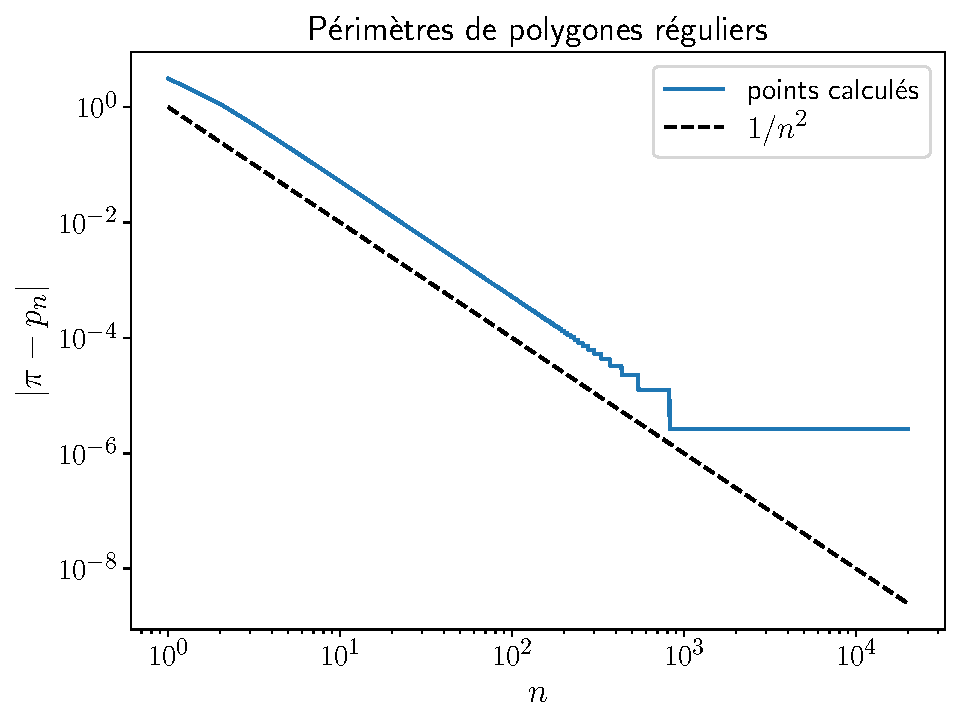
\includegraphics[width=0.45\paperwidth]{TD2/perimetres-polygones-reguliers.pdf}
\end{center}

Pourquoi, à votre avis, la courbe finit-elle ici en escalier au lieu de suivre une belle loi d'échelle ?

\end{correction}

\renewenvironment{correction}{}{}
\excludecomment{correction}

\section{La classe \mintinline{c++}{complexe}}
 
Dans le précédent TD, nous représentions un nombre complexe par sa partie réelle et sa partie imaginaire. Chaque fois que nous passions un nombre complexe en argument d'une fonction nous devions passer sa partie réelle et sa partie imaginaire... En utilisant le concept d'objet, créer une classe \inline{complexe} qui représente un nombre complexe. Transformer les fonctions \inline{affiche}, \inline{norme} et \inline{argument} écrites précédemment afin que ces dernières soient des membres de la classe \inline{complexe}. On n'oubliera pas le mot-clé \inline{public}, et on pourra se renseigner sur la fonction \href{http://en.cppreference.com/w/cpp/numeric/math/atan2}{\inline{atan2}} de \inline{<cmath>}. Bien évidemment, on testera le code écrit.

\begin{correction}

On défini ensuite la classe \inline{complexe} de la manière suivante, dans \filename{complexe.h} (le mot-clé \inline{public} est essentiel ; par défaut les membres et méthodes d'une classe sont privés (\inline{private}), non accessibles depuis l'extérieur de la classe)
\begin{minted}[breaklines]{c++}
#ifndef COMPLEX_H
#define COMPLEX_H

class complexe {
public:
  double re, im;

  void affiche();

  double norme();
  double argument();
};

#endif // COMPLEX_H
\end{minted}
Elle contient deux membres, la partie réelle et la partie imaginaire, et déclare les trois méthodes demandées par l'énoncé. On aura pris soin d'inclure le \emph{header guard}.

L'implémentation \emph{doit} être faite dans le fichier \filename{complexe.cpp} (en général, sauf pour les méthodes dites en ligne, \inline{inline}). On commence par inclure les fichiers d'en-tête donnant accès à la classe \inline{complexe}, à \inline{cout} et aux fonctions mathématiques
\begin{minted}[breaklines]{c++}
#include "complexe.h"

#include <iostream>
#include <cmath>
using namespace std;
\end{minted}
Puis on définit les méthodes de la classe \inline{complexe} dans \filename{complexe.cpp}
\begin{minted}[breaklines]{c++}
void complexe::affiche() {
  cout << re << " + " << im << " i" << endl;
}

double complexe::norme() {
  return sqrt(re*re + im*im);
}

double complexe::argument() {
  return atan2(im, re);
}
\end{minted}
On n'oubliera pas la résolution de portée \inline{complexe::} devant le nom des méthodes.

Finalement, on teste ce qu'on vient d'écrire dans \filename{main.cpp}:
\begin{minted}[breaklines]{c++}
#include <iostream>
using namespace std;

#include "complexe.h"

int main()
{
  complexe a;

  a.re = sqrt(2);
  a.im = sqrt(2);

  a.affiche();

  cout << "Norme : " << a.norme() << endl;
  cout << "Argument :" << a.argument() << " (" << 180.0 * a.argument() / M_PI << "deg)" << endl;

  return 0;
}
\end{minted}

On n'oubliera pas de modifier le \filename{makefile}.

\end{correction}

\section{La fonction exponentielle}
Déclarer et définir une fonction \emph{non-membre} \inline{exponentielle(complexe)} qui prend en argument un nombre complexe et qui renvoie un nombre complexe.

\begin{correction}
Comme nous avons une classe \inline{complexe} à notre disposition, nous pouvons retourner le résultat d'une opération via \inline{return} au lieu de devoir passer des argument par référence. La fonction \inline{exponentielle} a pour déclaration (dans \filename{complexe.h})
\begin{minted}[breaklines]{c++}
complexe exponentielle(complexe a);
\end{minted}
et pour définition (dans \filename{complexe.cpp})
\begin{minted}[breaklines]{c++}
complexe exponentielle(complexe a)
{
  complexe result;

  result.re = exp(a.re) * cos(a.im);
  result.im = exp(a.re) * sin(a.im);

  return result;
}
\end{minted}
Comme la fonction \inline{exponentielle} n'est pas une fonction membre de la classe \inline{complexe}, il n'y a pas d'opérateur de résolution de portée \inline{complexe::} lors de la définition de la fonction dans le fichier \inline{complexe.cpp}

Sans rien changer à la définition de \inline{exponentielle} (mis à part la signature de la fonction), nous aurions pu la déclarer de la manière suivante
\begin{minted}[breaklines]{c++}
complexe exponentielle(const complexe & a);
\end{minted}
Cette définition signifie que l'argument est passé par référence, mais que l'utilisateur de la fonction est assuré que la valeur de l'argument ne sera pas modifié par la fonction.\\

\end{correction}

\section{Tableaux de complexes}

Dans le TD précédent (exercices 1.6 et 1.7), nous avons utilisé des tableaux de parties réelles et imaginaires. Ré-écrire le programme de l'exercice 1.6 ou 1.7 du TD1 en utilisant la classe \inline{std::vector<complexe>}.\\

Rappel de méthodes qui peuvent être utiles :
\begin{itemize}
  \item \inline{vector<complexe> monTableau;} pour déclarer un tableau contigu d'objets de type \inline{complexe}.
  \item \inline{monTableau.push_back(nombre)} pour rajouter le un nombre à la fin du tableau. La taille du tableau est ajustée automatiquement.
  \item \inline{monTableau.size()} pour connaître le nombre d'éléments dans le tableau.
  \item \inline{monTableau[i]} ou \inline{monTableau.at(i)} permet d'accéder au $i$-ème élément du tableau (possiblement pour le modifier). Comme corollaire évident :
  \begin{itemize}
    \item Si la classe \inline{complexe} possède une méthode \inline{truc()}, \inline{monTableau[i].truc();} permet d'appeller la méthode \inline{truc()} sur le $i$-ème élément du tableau. On peut aussi utiliser \inline{monTableau.at(i).affiche();} si la méthode \inline{affiche()} a été déclarée \inline{const}),
    \item Si la classe \inline{complexe} possède un membre nommé \inline{re}, \inline{monTableau[i].re = 1.2;} permet de modifier la valeur du membre \inline{re} du $i$-ème nombre complexe du tableau.
  \end{itemize}
\end{itemize}
 
\begin{correction}
On commence par inclure la bibliothèque \inline{<vector>}, et on s'assure d'utiliser l'espace de nom \inline{std}.
\begin{minted}[breaklines]{c++}
#include <vector>
using namespace std;
\end{minted}

Ici on ne fait pas d'allocation de mémoire à la main; on déclare simplement un tableau automatique \inline{vector<complexe>}. 
\begin{minted}[breaklines]{c++}
int main() 
{
  unsigned int N = 0;
  cout << "N = ";
  cin >> N;

  vector<complexe> nombres;
\end{minted}

Pour remplir le tableau avec $e^{\frac{2i\pi n}{N}}$, nous allons faire appel à la fonction \inline{exponentielle}; nous créons donc d'abord le nombre complexe $0 + \frac{2i\pi n}{N}$, puis nous ajoutons l'exponentielle de ce nombre à la fin du tableau grâce à \inline{push_back}.
\begin{minted}[breaklines]{c++}
  for (unsigned int n = 0; n < N; ++n) {
    complexe nombre;
    nombre.re = -0.4242; // parce ça ne change rien, pourquoi pas
    nombre.im = 2 * n * M_PI / N;
    
    nombres.push_back(exponentielle(nombre));
  }
\end{minted}

Finalement, nous accédons aux parties réelles et imaginaire des nombres complexes du tableau afin de calculer leur somme
\begin{minted}[breaklines]{c++}
int main () {
  complexe somme;
  somme.re = 0;
  somme.im = 0;
  
  for (unsigned int n = 0; n < nombres.size(); ++n) {
    // deux façons différentes d'accéder à un élément d'un vector :
    somme.re += nombres[n].re;  // accès par indice
    somme.im += nombres.at(n).im;   // accès avec la méthode .at(n), qui vérifie en plus si n est un indice valide et affiche une erreur sinon (plus sécurisé mais un tout petit peu plus lent)
  }

  somme.affiche();

  return 0;
}
\end{minted}
On remarque que grâce à l'utilisation de la classe \inline{complexe}, le code est plus court et plus simple. On verra plus tard que, avec la surcharge d'opérateurs, on pourra écrire un code encore plus concis.
\end{correction}

%--------------------------------------------------------------------------------

\section{Surcharge d'opérateurs}

\emph{Pré-requis : cours 5 sur la surcharge d'opérateurs.}\\

Cette partie a pour but d'introduire la notion de surcharge d'opérateur afin de pouvoir écrire des expressions naturelles du type \inline{complexe moins_un = complexe(0,1) * complexe(0,1)}.\\

Nous allons surcharger les opérateurs binaires (c'est-à-dire prenant deux arguments) comme \inline{operator+}, \inline{operator*}, ainsi l'opérateur unaire (c'est-à-dire prenant un seul arguments) \inline{complexe operator-(complexe)}. Il y a deux façons de faire :
\begin{enumerate}
\item Déclarer les opérateurs comme des fonctions et non des membres de la classe \texttt{complexe}. Ils prennent alors tous leurs opérandes par argument. Exemple : \inline{complexe operator+ (complexe a, complexe b)}. C'est la façon la plus intuitive. On pourra soit les déclarer à l'extérieur de la classe \inline{complexe}, soit les déclarer comme fonctions amies\footnote{Les fonctions amies ne sont pas au programme du cours mais il est possible de tomber sur du code les utilisant. Pour faire bref : une fonction amie n'est pas une fonction membre (même s'il faut la déclarer à l'intérieur de la classe avec le mot clé \inline{friend} en préfixe), mais elle a accès aux attributs privés de la classe. Ceci ne fera sens pour vous que dans la suite du cours. Pour l'instant tous les attributs sont publiques, ça ne change donc rien.} à l'intérieur de la classe \inline{complexe}. On parle de \textit{non-member operator overloading}.
\item Déclarer les opérateurs comme méthodes membres de la classe \texttt{complexe}, prennant un unique argument \texttt{complexe}. Le premier opérande est implicitement l'objet lui même, ie. \inline{*this}, et le deuxième opérande est l'argument. Exemple : \inline{complexe complexe::operator+ (complexe b) const}. On parle de \textit{member operator overloading}.
\end{enumerate}
Ces deux façons sont équivalentes dans la plupart des cas. Une exception : si \texttt{a} n'est pas un \texttt{complexe} mais est \emph{convertible en \texttt{complexe}} (par exemple \inline{1 + complexe(0,1)}), l'opération sera valide avec du \textit{non-member overloading}, alors qu'elle ne le sera pas avec du \textit{member overloading}. Autre exemple : la multiplication scalaire à gauche, comme \inline{2 * complexe(0,1)}, ne peut pas être implémenté comme membre de la classe \texttt{complexe}. En général, il faut imaginer les cas d'utilisation et choisir la façon qui ne pose le moins de problèmes.\\

Nous allons également surcharger les opérateurs membres comme \inline{operator+=} ou \inline{operator*=}. Ces opérateurs ont une signature du type ou \inline{complexe& operator+= (const complexe&)}, et \emph{sont} des fonctions membres, il faut donc utiliser l'opérateur de résolution de portée \inline{complexe::} lors de la définition. Rappel : ces opérateurs de modifications renvoient non pas \inline{void}, mais \inline{complexe&}, renvoyant une référence sur soi-même. Ceci pour permettre d'écrire des expressions tordues comme \inline{(a *= 2) *= 3;} ou \inline{f(a += 1);}. Pour cela, il faut renvoyer \inline{*this}. Ce n'est pas bien grave si vous ne voyez pas l'intérêt pour le moment. Pour d'autres opérateurs (par exemple l'affectation, cf. suite du cours), cela devient clair.\\

Les opérations effectuées ici sont très rapide à écrire. Mais pour des opérations un peu plus complexes et lorsque l'on choisit le \textit{non-member operator overloading}, il est avantageux ou même nécessaire\footnote{lorsque des attributs privés de la classe sont en jeu (cf. cours suivant)} d'implémenter l'opération dans (par exemple) \inline{operator+=} et de simplement utiliser \inline{+=} dans le corps de \inline{complexe operator+ (complexe a, complexe b)}.\\

Définir les opérateurs \inline{operator+=} et \inline{operator-=} (argument \inline{complexe}), ainsi que \inline{operator*=} avec argument \inline{complexe} ou scalaire (\inline{double}). Pour les opérateurs binaire, afin d'explorer les différentes façon de faire :
\begin{itemize}
  \item définir les additions et multiplications entre deux complexes comme fonctions externes
  \item définir la multiplication entre un scalaire et un complexe, aussi bien à droite qu'à gauche, de la façon qui vous parait la plus appropriée
  \item définir les soustractions et divisions entre deux complexes comme méthodes de la classe \inline{complexe}
  \item définir l'opération d'inversion de signe (unaire, pour écrire par exemple \inline{complexe b = -a;}) comme méthode
\end{itemize}

Bien sûr, tester chacune de ces opérations. Enfin, on adaptera le code de l'exercice précédent afin d'utiliser les opérateurs surchargés.

\begin{correction}

\begin{minted}[breaklines]{c++}
class complexe
{
public:
  ...
  // addition de `b' à soi
  complexe& operator+= (complexe b);
  // soustraction de `b' à soi
  complexe& operator-= (complexe b);
  // multiplication de `b' à soi
  complexe& operator*= (complexe b);
  complexe& operator*= (double b);
  // division de soi par `b' :
  complexe& operator/= (complexe b);
  complexe& operator/= (double b);
  // opposé de soi
  complexe operator- () const;
  // soustraction de `a' et `b'
  complexe operator- (complexe b) const;
  // division de `a' par `b' :
  complexe operator/ (complexe b) const;
  complexe operator/ (double b) const;  // note: non demandé dans l'énoncé, mais utile
  ...
};

// multiplication de `a' par `b' (que `a' et `b' soient scalaires ou complexes)
complexe operator* (complexe a, complexe b);
complexe operator* (complexe a, double b);
complexe operator* (double a, complexe a);

// addition de `a' et `b'
complexe operator+ (complexe a, complexe b);
\end{minted}

Pour les opérateurs membres, l'implémentation est directe et ressemble à :

\begin{minted}[breaklines]{c++}
complexe& complexe::operator+= (complexe right) {
  re += right.re;
  im += right.im;
  return *this;
}

complexe& complexe::operator*= (double scalar) {
  re *= scalar;
  im *= scalar;
  return *this;
}
\end{minted}

De même pour la autres opérations à soi. Nous pouvons aussi prendre le parti d'utiliser les opérations binaires externes pour définir les opérations à soi. Par exemple :

\begin{minted}[breaklines]{c++}
complexe& complexe::operator*= (complexe right) {
  *this = (*this) * right;
  return *this;
}
\end{minted}

Ce n'est cependant en général pas recommandé pour des raisons de performance (copie inutile, que le compilateur peut cependant souvent optimiser). On implémente alors la multiplication dans la fonction externe :

\begin{minted}[breaklines]{c++}
complexe operator* (complexe a, complexe b) {
  complexe c;
  c.re = a.re * b.re - a.im * b.im;
  c.im = a.re * b.im + a.im * b.re;
  return c;
}
\end{minted}

Notons que nous avons pris les arguments par copie. Il est possible, et même recommandé pour éviter des copies inutiles,  de prendre les objets \inline{complexe} par référence constante :
\begin{minted}[breaklines]{c++}
class complexe {
  ...
  complexe& operator+= (const complexe& b);
  ...
};

complexe operator* (const complexe& a, const complexe& b);
...
\end{minted}
Toutefois, par souci de clarté, on a gardé un passage par copie dans cette correction. Un objet de type \inline{complexe} ne prennant que $2\times 8$ octets (contre $8$ pour un pointeur ou référence), la différence de performance est probablement peu perceptible, d'autant plus que le compilateur effectue certaines optimisations.\\

Pour les opérateurs non-membres, on peut simplement faire :

\begin{minted}[breaklines]{c++}
complexe operator+ (complexe a, complexe b) {
  complexe c;
  c.re = a.re + b.re;
  c.im = a.im + b.im;
  return c;
}
\end{minted}

Mais il est possible de faire plus efficace en évitant la création d'un intermédiaire :

\begin{minted}[breaklines]{c++}
complexe operator+ (complexe a, complexe b) {
  a.re += b.re;
  a.im += b.im;
  return a;
}
\end{minted}

Ici, on a pris l'argument \inline{a} par copie, on peut donc le modifier sans rirsque de modifier la variable de l'utilisateur ! Grâce à notre définition de \inline{complexe::operator+=(complexe)}, il est possible d'être encore plus expéditif :

\begin{minted}[breaklines]{c++}
complexe operator+ (complexe a, complexe b) {
  return (a += b);
}
\end{minted}

Noter que l'on a renversé les rôles par rapport à notre implémentation de la multiplication ci-dessus : c'est \inline{operator+} qui utilise \inline{operator+=} et non l'inverse. C'est la façon de faire recommandée, et même nécessaire lorsqu'on agit sur des attributs privés (cf. cours suivant).\\

Finissons avec les divisions, toutes définies comme méthodes :
\begin{minted}[breaklines]{c++}
complexe& complexe::operator/= (double scalar) {
  re /= scalar;
  im /= scalar;
  return *this;
}

complexe complexe::operator/ (double scalar) const {
  return { re/scalar, im/scalar };
}

complexe complexe::operator/ (complexe right) {
  return (*this) * right.conj() / right.abssquare();
}

complexe& complexe::operator/= (complexe right) {
  // parce que l'on est un peu paresseux :
  *this = (*this) / right;
  return *this;
}
\end{minted}

Notons que nous avons pris la liberté, pour clarifier l'implémentation de la division, de définir deux méthodes \inline{complexe::conj()} et \inline{complexe::abssquare()}, déclarées comme suit :
\begin{minted}[breaklines]{c++}
class complexe {
  ...
  complexe abssquare () const;
  complexe conj () const;
  ...
};
\end{minted}
et définies ainsi :
\begin{minted}[breaklines]{c++}
complexe complexe::abssquare () const {
  return re * re + im * im;
}

complexe complexe::conj () const {
  return { re, -im };
}
\end{minted}

On note l'utilisation de l'initialisation de structures "à la C" (\inline{complexe {re, im}}), qui sera remplacé par la notion bien plus générale de \emph{constructeur} (et qui ne dépend pas de l'ordre dans lequel sont définit les attributs) dans la suite du cours.

\end{correction}

\section{L'opérateur de flux \mintinline{c++}{<<}}
L'opérateur de flux \inline{operator<<} peut également être surchargé pour pouvoir écrire
\begin{minted}[breaklines]{c++}
complexe i(0,1);
cout << i << endl;
\end{minted}
On l'utilise ici comme un opérateur binaire dont l'opérande de gauche est \inline{cout} et dont l'opérande de droite est notre nombre complexe. La signature à utiliser est alors \inline{std::ostream& operator<< (std::ostream& out, const complexe& nombre)}. En effet, \inline{std::cout} est un objet de type \inline{std::ostream} spécialement implémenté pour afficher dans la console\footnote{D'ailleurs, \inline{std::ofstream} étant aussi de type \inline{std::ostream}, cette surcharge de \inline{operator<<} fonctionnera aussi pour l'écriture de fichiers. Même chose pour \inline{std::ostringstream}.}.\\

Pourquoi renvoit-on une référence sur le flux \inline{out} que l'on prend en argument, au lieu de \inline{void} ? Simplement pour pouvoir chaîner les opérations d'affichage (ie. \inline{cout << i << endl;} au lieu de \inline{cout << i; cout << endl}).

\begin{correction}
Dans \filename{complexe.h}, assurons-nous d'abord que le type \inline{ostream} est déclaré, via
\begin{minted}[breaklines]{c++}
#include <ostream>
\end{minted}
Ensuite il faut déclarer l'opérateur de flux via
\begin{minted}[breaklines]{c++}
std::ostream& operator<< (std::ostream& out, const complexe& nombre);
\end{minted}
%Nous ne sommes pas obligés de déclarer cette fonction dans la classe \inline{complexe} précédée du mot-clé \inline{friend} car pour afficher un nombre complexe dans la console nous pouvons nous contenter d'utiliser les membres \inline{public} de la classe. (De manière générale, quand on affiche un objet dans la console, on n'a pas besoin d'afficher des informations qui ne sont pas visibles par l'utilisateur, ie. \inline{private}.)

On notera l'utilisation de \inline{std::} car utiliser \inline{using namespace} à l'intérieur d'un fichier \filename{*.h} est une très mauvaise idée, et doit être évité, sinon, tous les fichiers qui incluent ce fichier \emph{*.h} subiront automatiquement l'usage de cet espace de nom.\\

Finalement, une possible implémentation de l'opérateur de flux peut-être
\begin{minted}[breaklines]{c++}
ostream& operator<< (ostream& out, const complexe& nombre) {
  if (nombre.imag() >= 0) {
    out << nombre.real() << " + " << nombre.imag() << "i";
  } else {
    out << nombre.real() << " - " << -nombre.imag() << "i";
 }
 return out;
}
\end{minted}
à écrire dans \filename{complexe.cpp} bien sûr. Ici, nous n'avons plus besoin d'utiliser \inline{std::} car nous sommes dans un fichier source \filename{*.cpp} dans lequel on aura pris soin d'insérer \inline{using namespace std;}. Ce n'est pas un problème ici, car un fichier \filename{*.cpp} ne peut pas être inclus dans un autre, donc l'instruction \inline{using namespace std;} a de l'effet uniquement à l'intérieur de ce fichier.\\
\end{correction}

%-----------------------------------------------------------------------------------

\newpage
\section{Méthode de Newton et fractales}

Concluons ce TD par une étude des propriétés de convergence de la méthode de Newton.\\

\subsection{Introduction}

La méthode de Newton permet de trouver numériquement un zéro d'une fonction $f(z)$, à condition de connaître sa dérivée $f'(z)$. Cette méthode est souvent présentée avec des fonctions réelles, mais elle est tout aussi bien applicable aux fonctions holomorphes.\\

Pour rappel, la méthode de Newton est une méthode itérative consistant à approximer la fonction $f(z)$ par sa linéarisation autour d'un point de travail $z_n$ :
\begin{equation*}
f(z) \simeq f(z_n) + (z-z_n)\,f'(z_n)
\end{equation*}
dont il est facile de connaitre le zéro $z^{(0)}$ (équation affine) :
\begin{equation*}
0 = f(z_n) + (z^{(0)} - z_n)\,f'(z_n) \quad \Leftrightarrow \quad z^{(0)} = z_n - \frac{f(z_n)}{f'(z_n)}
\end{equation*}
Dit autrement, $z^{(0)}$ est l'intersection de la tangeante de $f$ en $z_n$ avec l'axe des abscisses, comme le montre . Ce n'est évidemment pas un zéro de $f$, mais on a bon espoir que $z^{(0)}$ soit plus proche d'un zéro que $z_n$. On itère alors cette prodécure en prenant ce $z^{(0)}$ comme un nouveau point de travail :
\begin{equation*}
z_{n+1} = z_n - \frac{f(z_n)}{f'(z_n)}
\end{equation*}
en espérant converger vers un point fixe de cette relation de récurrence. Il est immédiat de voir que les points fixes de cette relation sont les zéros $z_\star$ de la fonction ($f(z_\star)=0$).

\begin{figure}[H]
\centering
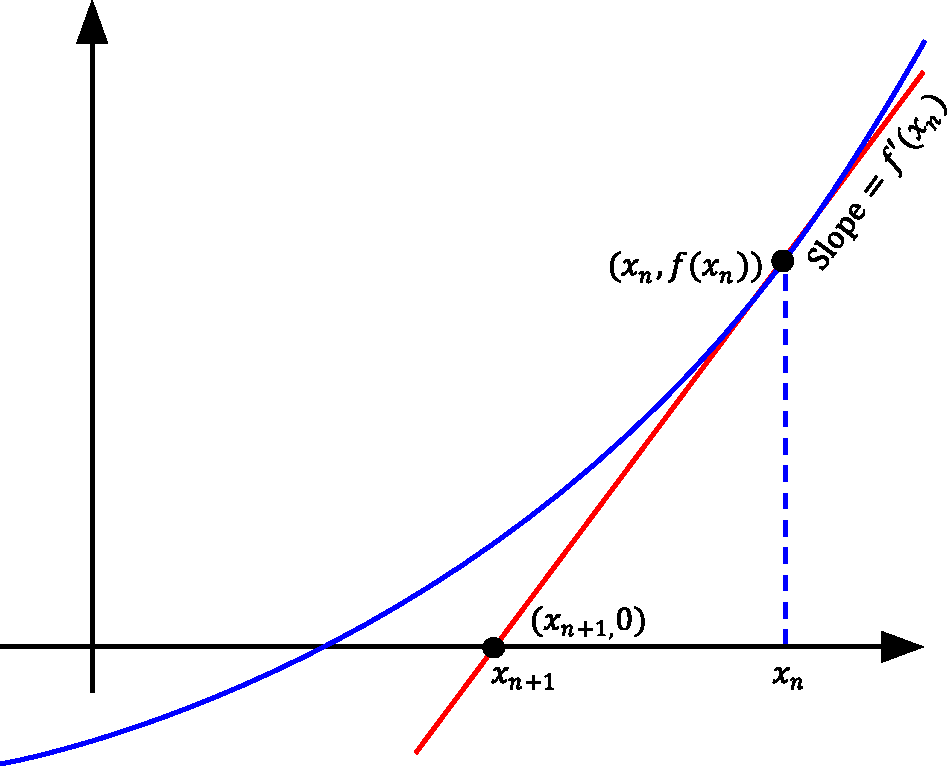
\includegraphics[width=0.5\linewidth]{TD2/newton_iteration.pdf}
\caption{Illustration d'une itération de la méthode de Newton sur une fonction réelle.}
\end{figure}

On peut montrer que dans un certain voisinage d'un zéro $z_\star$, la méthode converge bien : $z_n \xrightarrow[n\to\infty]{} z_\star$ pour tout point initial $z_0$ dans ce voisinage. Il est bien connu que la méthode de Newton converge extrêmement rapidement : si le zéro n'est pas aussi un point de rebroussement (ie. si $f'(z_\star) \neq 0$, alors \emph{on double le nombre de chiffres significatifs à chaque étape !}\\

Ceci dit, ce voisinage dépend fortement de la fonction. En dehors de ce voisinage, tout peut arriver : ça peut ne pas converger, ou ça peut converger vers n'importe quel autre zéro de la fonction. La vitesse de convergence peut bien évidemment dépendre du point de départ. C'est ce que nous voulons étudier.\\

\subsection{Implémentation}

Pour cela, nous voulons écrire une fonction \inline{methode_newton} effectuant cette prodédure (en n'allant bien sûr pas jusqu'à l'infini...), sur une fonction holomorphe $f$ quelconque. Il nous faut donc passer en argument une fonction à \inline{methode_newton}. Comment faire en C++ ?\\

Le "type" (ou plutôt conteneur standard) de fonction en C++ est \inline{std::function<...>}, dont l'argument template est le prototype de la fonction, sous forme \inline{type_de_retour(type_arg1,type_arg2,...)}. Ainsi, pour une fonction complexe, on peut utiliser \inline{std::function<complexe(complexe)>}. Pour éviter d'écrire de nombreuses fois ce type un peu long, on peut définir un alias, par exemple :
\begin{minted}[breaklines]{c++}
  #include <functional>
  using fonc_complexe_t = std::function<complexe(complexe)>;
\end{minted}
Un objet de type \inline{std::function} peut être appelé avec les parenthèses, comme n'importe quelle fonction.

Écrire une fonction de prototype
\begin{minted}[breaklines]{c++}
  std::tuple<complexe,int> methode_newton (
    fonc_complexe_t f,
    fonc_complexe_t f_deriv,
    complexe z_init,
    unsigned int max_it,
    double epsilon
  )
\end{minted}
où \inline{f} et \inline{f_deriv} sont $f$ et $f'$ respectivement, où \inline{z_init} est le point initial de l'itération, où \inline{max_it} est le nombre maximal d'itérations (pour arrêter les itérations au cas où ça ne converge pas), et où \inline{epsilon} est le seuil de convergence (lorsque $|f(z_{n_\text{fin}})|<\epsilon$, on dit que l'on a trouvé un zéro). La fonction \inline{methode_newton} retourne le zéro estimé $z_{n_\text{fin}}$ ainsi que le numéro d'itération $n_\text{fin}$ auquel l'algorithme a convergé, ou $-1$ autrement. On profitera des opérateurs surchargés précédemment pour simplifier l'écriture.\\

Ces deux informations sont retournées sous forme d'un tuple \inline{std::tuple<complexe,int>}. Pas de panique, c'est très simple à utiliser. On peut créer un tuple de la façon suivante :
\begin{minted}[breaklines]{c++}
  std::tuple<complexe,int> t = { complexe(0,1), 13 };
\end{minted}
Pour dépaqueter un tuple, on peut utiliser la syntaxe
\begin{minted}[breaklines]{c++}
  auto [z,n] = t;
\end{minted}
où les variables \inline{complexe z} et \inline{int n} sont déclarées puis assignées aux valeurs contenus dans le tuple.\\

Pour passer une fonction à \inline{methode_newton}, on peut
\begin{itemize}
  \item Soit déclarer une fonction de façon habituelle \inline{complexe f (complexe z);} puis simplement écrire \inline{f} comme argument.
  \item Soit créer une fonction lambda, par exemple
\begin{minted}[breaklines]{c++}
  std::function<complexe(complexe)> f = [] (complexe z) -> complexe {
    ...
  }; 
\end{minted}
  Il est aussi possible d'écrire directement la lambda en argument sans déclarer la variable \texttt{f} intermédiaire.
\end{itemize}

\vspace{1em}
N'hésitez pas à temporairement ajouter un affichage des valeurs durant l'itération pour voir ce qu'il se passe et observer la convergence. On pourra faire en sorte d'augmenter le nombre de chiffres affichés avec \inline{std::setprecision}. N'hésitez pas non plus à converger jusqu'à $10^{-25}$. Testez votre fonction sur, disons, $f(z)=z-1$ et $f(z)=(z-1)^2$ à partir d'un point relativement éloigné du zéro $z_\star=1$. Voyez-vous une différence de vitesse de convergence ? Pourquoi ?\\

\begin{correction}
Implémentation possible :

\begin{minted}[breaklines,samepage]{c++}
#include <iostream>

std::tuple<complexe,int> methode_newton (fonc_complexe_t f, fonc_complexe_t f_deriv, complexe z, unsigned int max_it, double epsilon, bool debug = false) {
  int n = 0;
  complexe fz = f(z);
  epsilon *= epsilon;
  // on regarde plutôt |f(z)|^2 < espilon^2
  while (fz.abssquare() > epsilon) {
    if (n >= max_it)
      return { z, -1 };
    z -= fz / f_deriv(z);
    n += 1;
    fz = f(z);
    if (debug)
      std::cout << "newton iter " << n << " : f(z) = " << fz << " at z = " << z << std::endl;
  }
  return { z, n };
}
\end{minted}

On observe une petite optimisation : on effectue la comparaison $|f(z)|^2 < \epsilon^2$ car la racine carrée nécessaire au calcul de $|f(z)|$ est coûteuse.\\

Notez qu'il n'y a aucun besoin de déclarer une variable locale complexe pour $z_n$, l'argument \inline{z} (passé par copie) fait très bien l'affaire. Par contre, comme $f(z)$ rentre à la fois dans le test de convergence et la relation de récurrence, autant définir une variable \inline{fz} pour éviter de le calculer deux fois par itération.\\

Enfin, on s'est permis d'ajouter un flag \inline{debug} pour activer l'affichage des itérations au besoin. Notre main ressemble à

\begin{minted}[breaklines,samepage]{c++}
#include <iomanip>

complexe f (complexe z) {
  complexe zm1 = (z-complexe(1,0));
  return zm1*zm1;
};

complexe f_deriv (complexe z) {
  return 2.*(z-complexe(1,0));
};

int main () {
  std::cout << std::setprecision(25) << std::fixed;
  complexe z_0 = {3,-10};
  auto [z_zero, nit] = methode_newton(f, f_deriv, z_0, 100, 1e-25, true);
  std::cout << z_zero << ", " << nit << std::endl;
  return 0;
}
\end{minted}

Pour $f(z)=(z-1)^2$, la convergence vers le zéro $z_\star=1$ est plus lente car $f'(z_\star) = 0$. On ne gagne qu'un chiffre de précision toutes les $\sim 4$ itérations. Autrement dit, la convergence est "seulement" exponentielle au lieu de super-exponetielle.
\end{correction}

%--------------------------

\subsection{Comportement fractal}

Dans la suite, nous allons étudier ce que donne la méthode de Newton sur un polynôme. Prenons par exemple $f(z)=z^3-1$, qui est un grand classique. Combien de zéro possède-t-il sur $\mathbb{C}$, et quels sont-ils ? Libre à vous d'en étudier un autre, ou même une fonction plus exotique, à conditions que vous connaissiez ses zéros.\\

\begin{correction}
De façon générale, les zéros de $f(z)=z^n-1$ sont les racines n-èmes de l'unité, $\{ \mathrm{e}^{2\pi \mathrm{i}\,k/n} \}_{0\leq k < n}$, au nombre de $n$. Pour $f(z)=z^3-1$, on a donc
  \begin{equation*}
  1,\quad \mathrm{e}^{2\pi \mathrm{i}/3}=\frac{-1+\mathrm{i}\sqrt{3}}{2},\quad \mathrm{e}^{2\pi \mathrm{i}\,2/3}=\frac{-1-\mathrm{i}\sqrt{3}}{2}
  \end{equation*}
Sa dérivée est $f'(z)=3 z^2$. Nous définissons
\begin{minted}[breaklines]{c++}
fonc_complexe_t f = [] (complexe z) { return z*z*z - complexe(1,0); };
fonc_complexe_t f_deriv = [] (complexe z) { return 3.*z*z; };
\end{minted}
Notons que le calcul \inline{z*z} est effectué deux fois par itération, ce qui n'est pas optimal. Ceci dit, il est possible que le compilateur le remarque et évite ce double calcul.
\end{correction}

Mettez-vous proche de $z_0=0$ et variez légèrement cette valeur de départ dans différentes direction. Sur quel zéro tombez vous ? Êtes-vous d'accord avec votre voisin ? Que fait le temps de convergence à mesure que l'on s'approche de zéro $z_0=0$ ? Pourquoi ?\footnote{Regardez $f'$...}\\

Pour y voir un plus clair, nous allons parcourir $z_0$ de façon systématique sur une grille de taille $N\times N$ maillant $\{x+\mathrm{i}y,\ x\in[-a,+a],\ y\in[-a,+a]\}$, et afficher le résultat avec matplotlib. Nous allons numéroter chaque zéro ainsi que lui définir une couleur, afin d'afficher une carte des bassins de convergence (ie. l'ensemble des points qui convergent vers un zéro donné).\\

Pour chaque point de la grille, exécutez la méthode de Newton et déterminez sur quel zéro la méthode a convergé. Choisissez $-1$ lorsqu'il n'y a pas eu convergence. Pour stocker les résultats, au lieu de définir des matrices dans notre programme, nous pouvons écrire directement dans un fichier lisible par \texttt{numpy.loadtxt}. Écrivez donc le numéro du zéro obtenu au fur et à mesure dans un fichier, en respectant le format demandé par \texttt{numpy.loadtxt} (c'est à dire une grille, avec des espaces horizontalement et des retours à la ligne verticalement). Compilez avec le flag \texttt{-O3} pour activer les optimisations du compilateur.\\

\begin{correction}
On a simplement à effectuer deux boucles imbriquées, en effectuant des pas $da=a/N$ sur la partie réelle et imaginaire de $z_0$ :
\begin{minted}[breaklines,samepage]{c++}
#include <fstream>

int main () {
  std::ofstream fichier_bassins_converg ("newton_bassins_converg.txt");

  fonc_complexe_t f = [] (complexe z) { return z*z*z - complexe(1,0); };
  fonc_complexe_t f_deriv = [] (complexe z) { return 3.*z*z; };
  constexpr unsigned int n_zeros = 3;
  complexe zeros [n_zeros] = { {1,0}, {-1/2.,sqrt(3)/2}, {-1/2.,-sqrt(3)/2} };

  int N = 1000;
  double a = 1.0, da = a/N;

  for (int i = -N; i <= N; i++) {
    for (int j = -N; j <= N; j++) {

      complexe z_0 = {i*da, j*da};
      auto [z_zero, nit] = methode_newton(f, f_deriv, z_0, 50, 1e-15, false);

      // détermination du numéro du zéro
      int num_zero = -1;
      for (int k = 0; k < n_zeros; k++) {
        if ((z_zero-zeros[k]).abssquare() < 1e-10)
          num_zero = k;
      }

      fichier_bassins_converg << num_zero << " ";
    }
    fichier_bassins_converg << "\n";
    std::cout << i << std::endl;
  }

  return 0;
}
\end{minted}

On utilise \inline{std::ofstream} pour écrire dans un fichier.

Note : nous avons omis \inline{fichier_bassins_converg.close()}. C'est tout à fait acceptable, le fichier est automatiquement fermé lorsque la variable \inline{fichier_bassins_converg} est détruite. Nous allons voir comment cela fonctionne dans la suite du cours.

\end{correction}

Avec Python, lire la grille résultante et la transformer en une image RBG, c'est-à-dire une grille de taille \inline{(N,N,3)}. Ainsi, \inline{img[42,24,:]} correspond au pixel $(42,24)$, et vaut \inline{[r,g,b]} où \texttt{r}, \texttt{g}, \texttt{b} sont entre $0$ et $1$ (\inline{[0,0,0]} pour du noir, \inline{[1,1,1]} pour du blanc). Pour les points qui n'ont pas convergés, choisir du noir par exemple. Astuce : forcer \texttt{dtype=int} pour \texttt{numpy.loadtxt} et utiliser des constructions du type \inline{img[ carte == ..., : ]} pour générer l'image. Ensuite, \inline{plt.imshow} permet d'afficher directement cette image. On prendra soin d'utiliser l'argument \texttt{extent} pour mettre les axes à la bonne échelle.\\

On obtient une magnifique fractale, la \emph{fractale de Newton}. Une caractéristique typique des fractales est l'auto-similarité. Vérifiez que notre fractale est bien auto-similaire, par exemple en dézoomant ou en zoomant autour du point $z_0=0$, et en zoomant encore, et encore, et encore...\\

\begin{correction}
\begin{minted}[breaklines,samepage]{python}
import numpy as np
import matplotlib.pyplot as plt

Iz = np.loadtxt("newton_bassins_converg.txt", dtype=int)
RGB = np.zeros((Iz.shape[0],Iz.shape[1],3))
Iz = Iz.transpose()[::-1,:]

RGB[ Iz == 0, : ] = [1,0,0]
RGB[ Iz == 1, : ] = [0.7,0,0.7]
RGB[ Iz == 2, : ] = [0,0,1]

a = 1.0
plt.figure(figsize=(10,10))
plt.imshow(RGB, extent=[-a,a,-a,a])
plt.show()
\end{minted}

La seule subtilité est au niveau de \texttt{Iz.transpose()[::-1,:]}. C'est nécessaire pour deux raisons : transposition parce que imshow n'a pas l'orgine standard, et inversion de l'axe vertical car on a parcouru de bas en haut.\\

Voici les bassins de convergence de la méthode de Newton pour les trois zéros de $z^3-1$, pour $a=10$, $a=1$, $a=0.1$ et $a=0.01$ :
\begin{center}
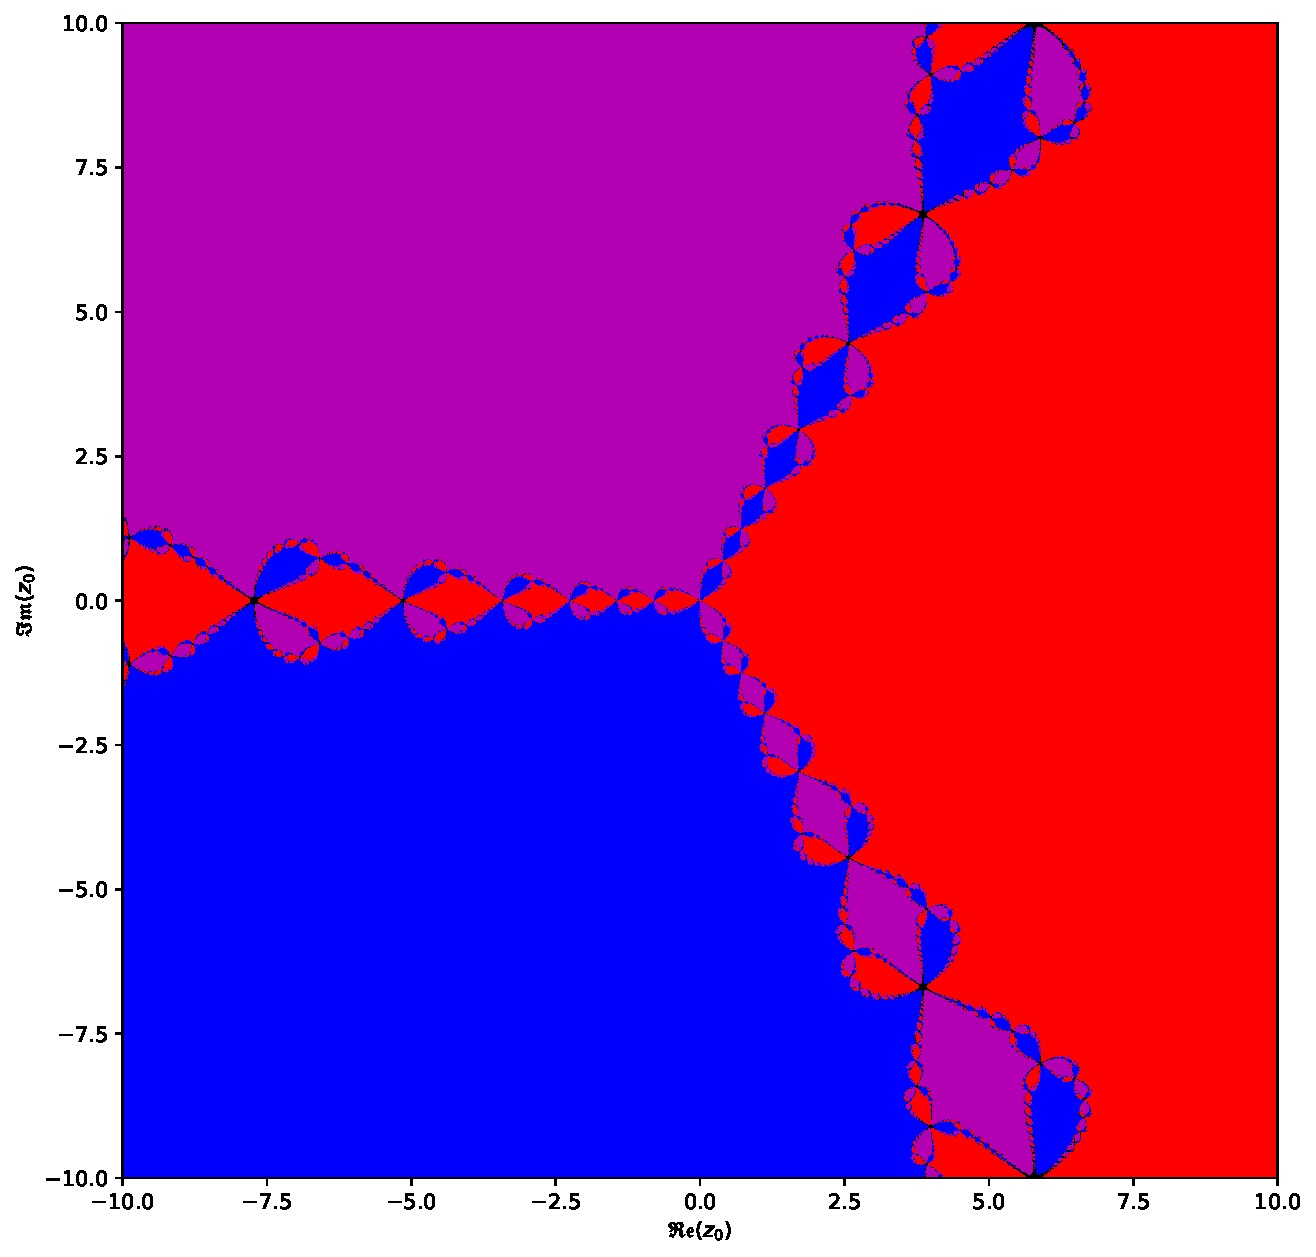
\includegraphics[width=0.49\linewidth]{TD2/newton_bassins_converg.a10.pdf}
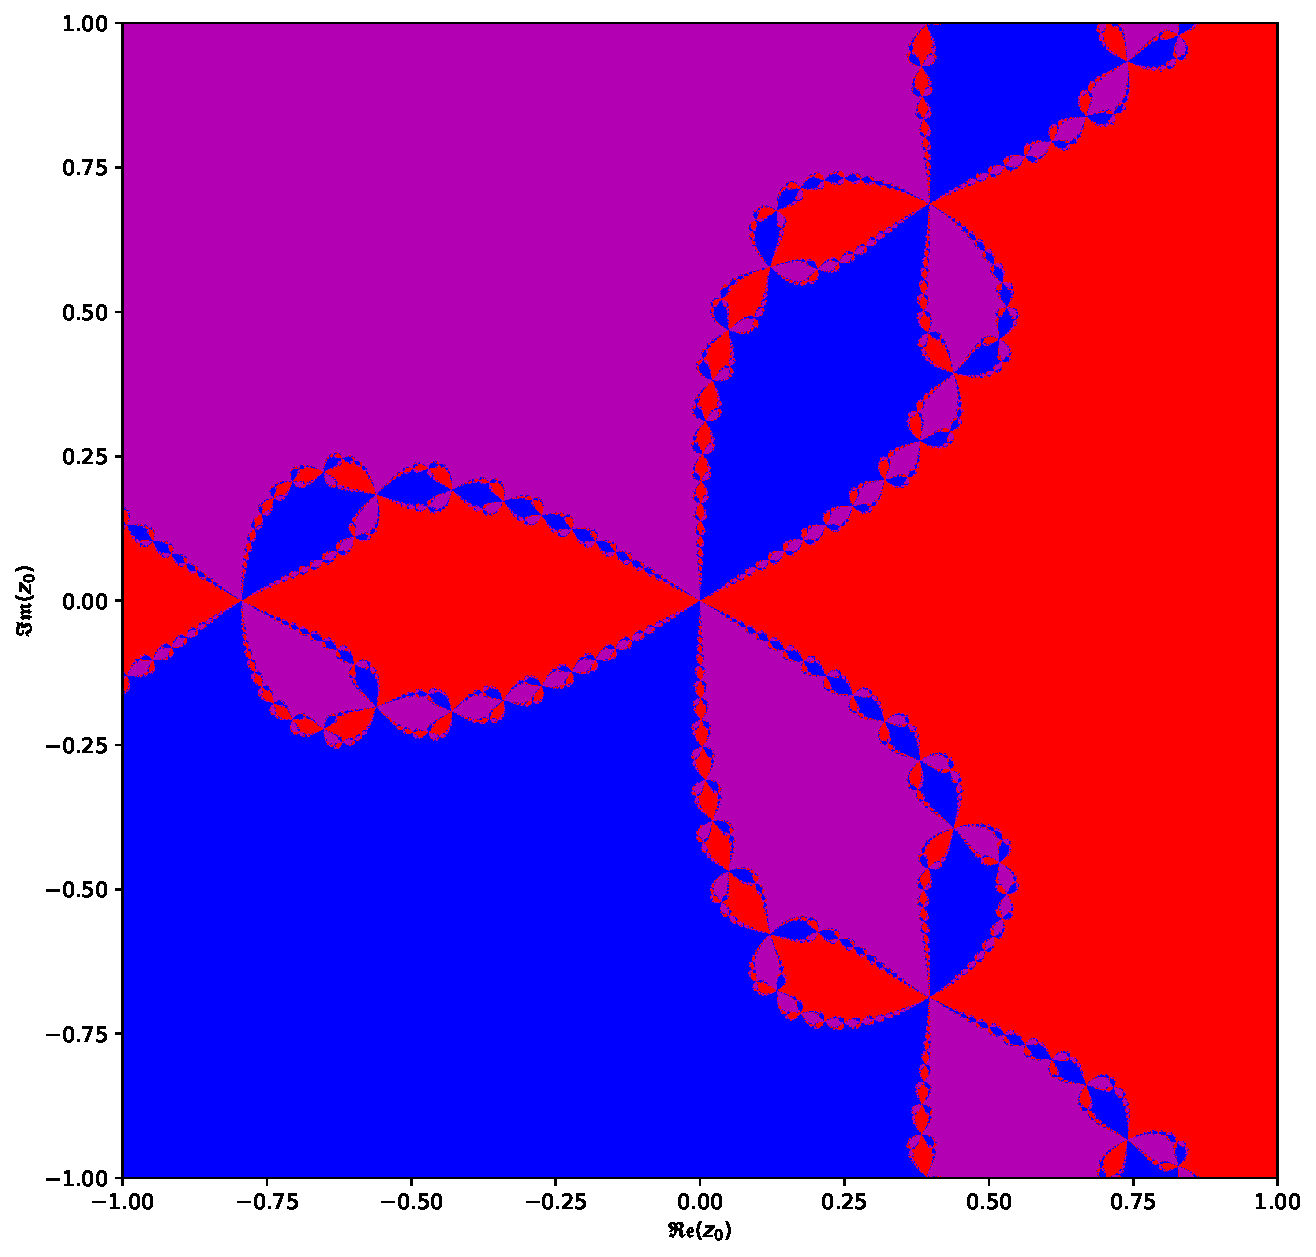
\includegraphics[width=0.49\linewidth]{TD2/newton_bassins_converg.a1.pdf}
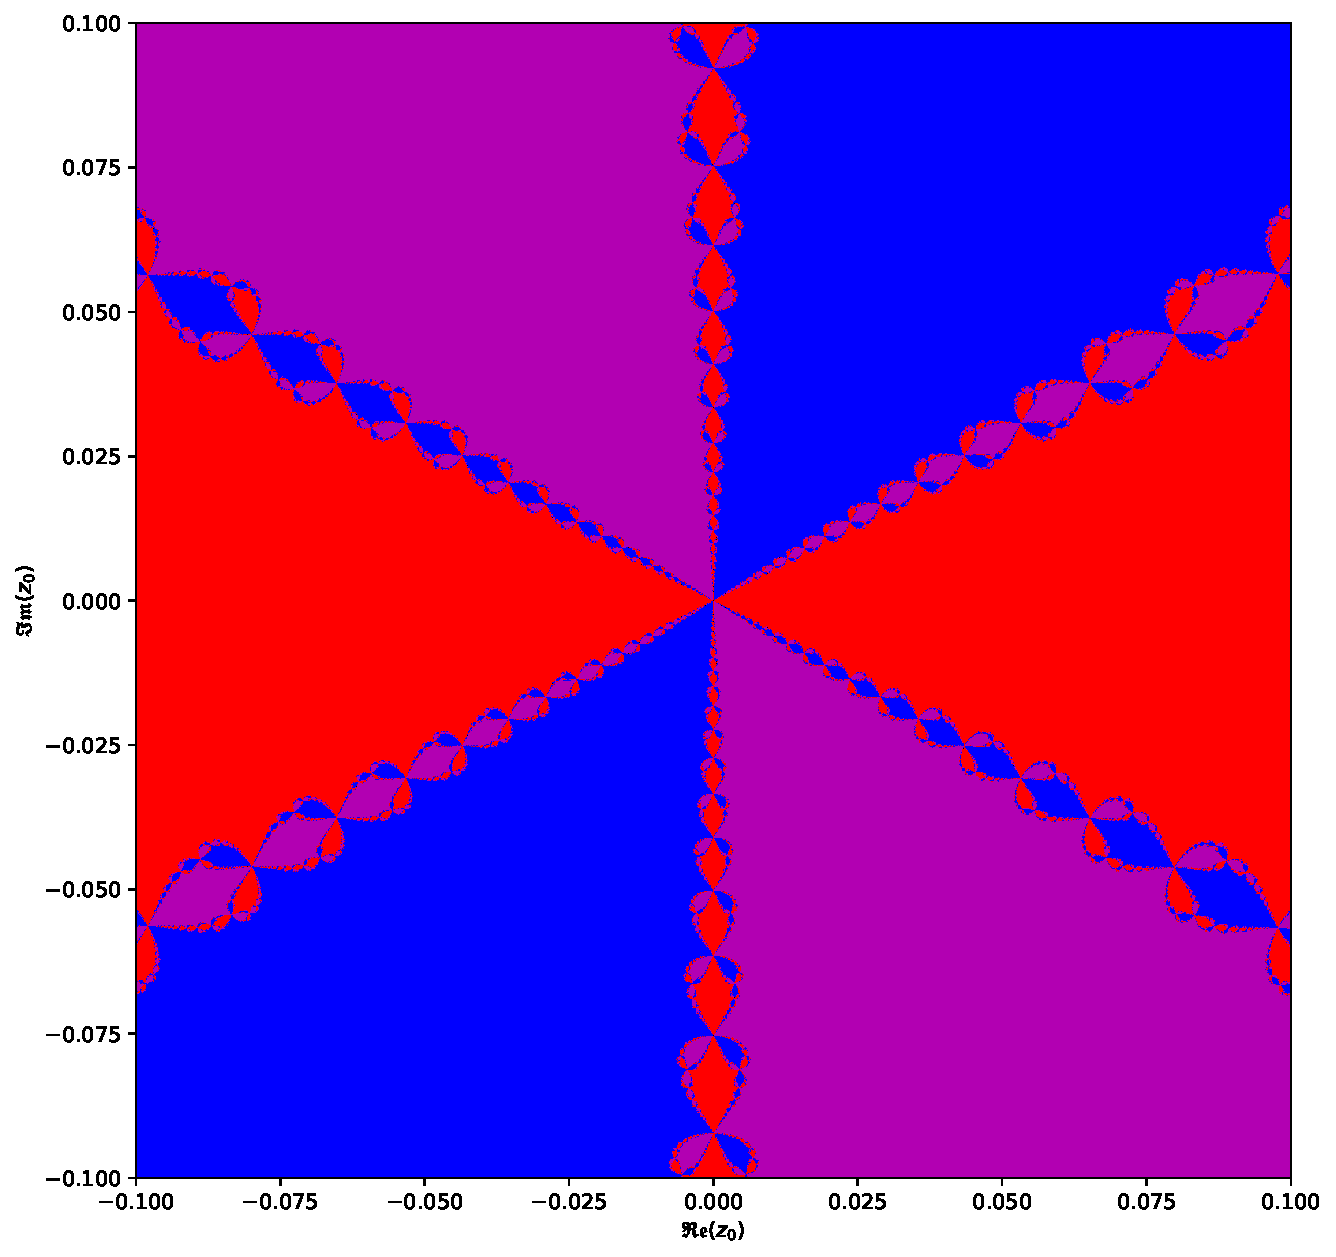
\includegraphics[width=0.49\linewidth]{TD2/newton_bassins_converg.a01.pdf}
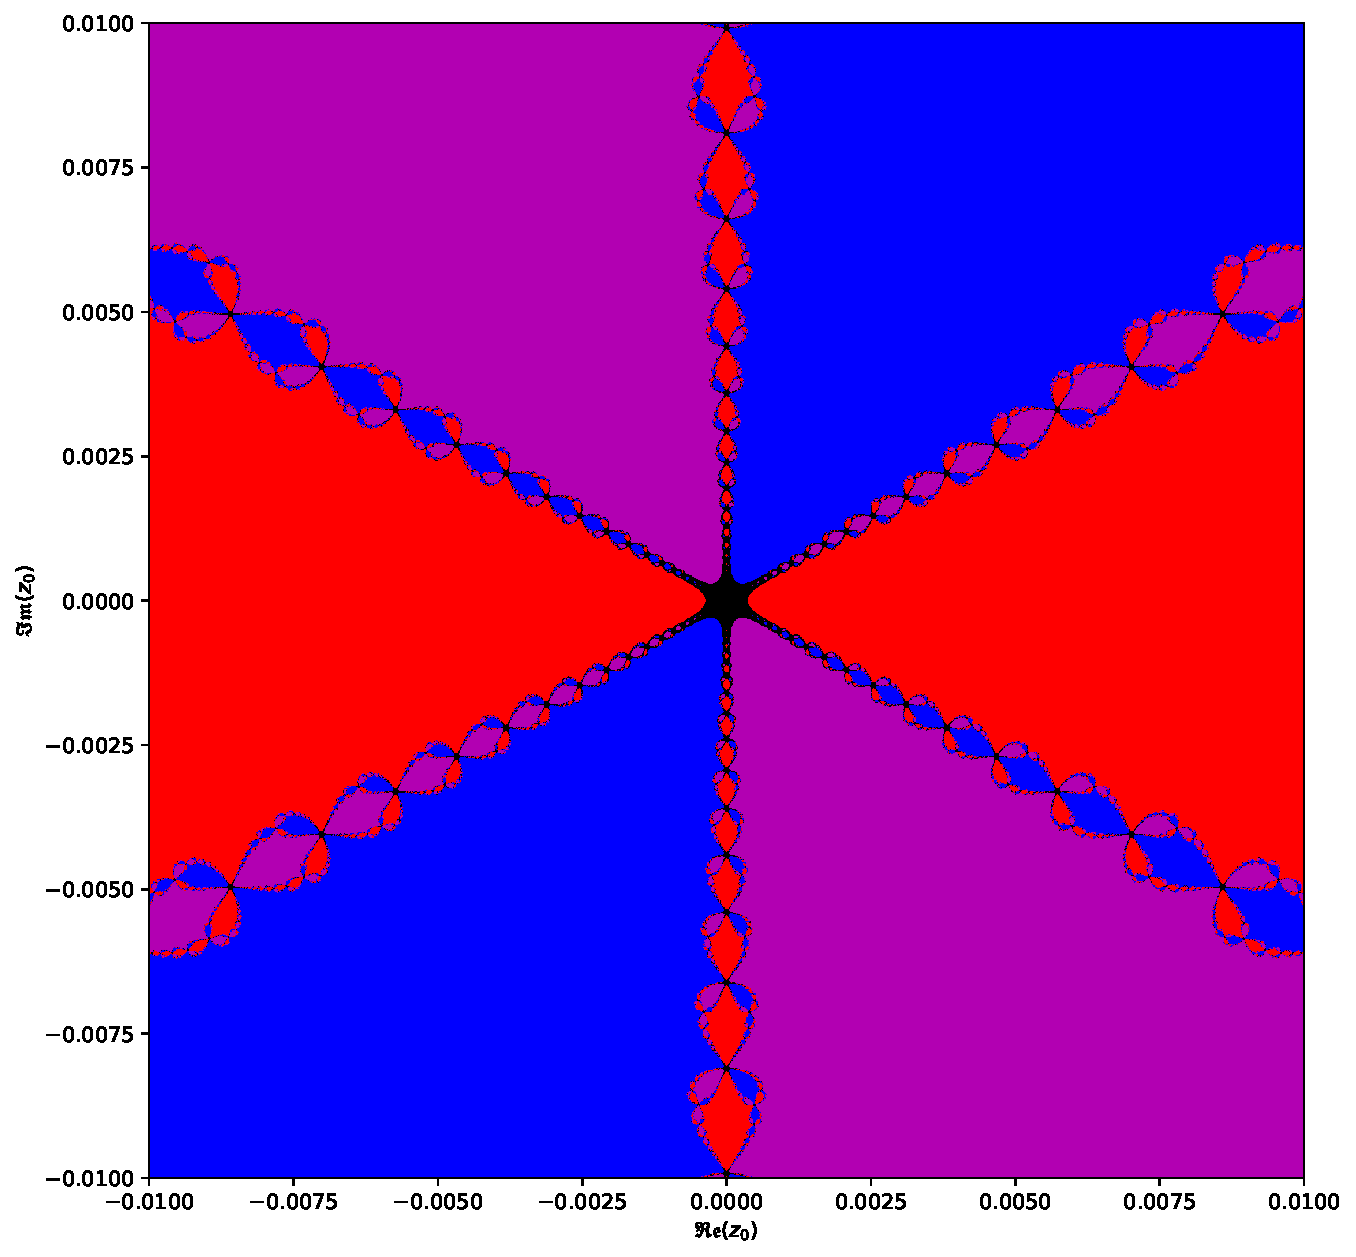
\includegraphics[width=0.49\linewidth]{TD2/newton_bassins_converg.a001.pdf}
\end{center}
chaque zéro ayant sa couleur. On a bien une auto-similarité, quoi que différente à grande échelle (3 "bras" pour $|z|>1$) qu'à petite échelle (6 "bras" pour $|z|<1$). Une remarque un petit défaut de convergence pour $a=0.01$, simplement car \inline{max_it} était un peu faible (40). Sans rentrer dans les détails, tentez d'intuiter la raison de cette auto-similarité en pensant à la trajectoire de $z_n$. Voici une trajectoire :
\begin{center}
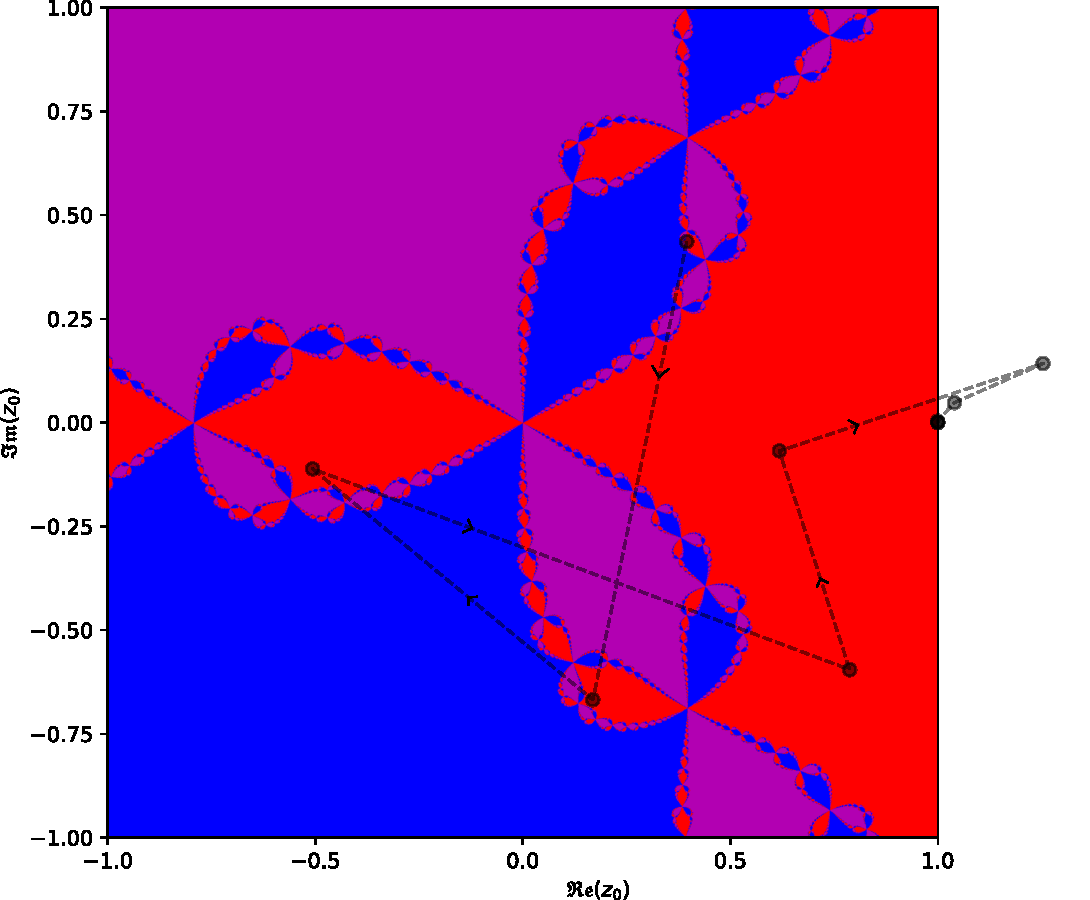
\includegraphics[width=0.7\linewidth]{TD2/newton_bassins_converg.a1_and_traj.pdf}
\end{center}
\end{correction}

Pour les motivés, on peut afficher une autre carte, possiblement plus belle encore, celle du nombre d'itérations nécessaires pour atteindre le seuil de convergence, $n_\text{fin}(z_0)$. Au lieu de créer une carte RBG, affichez directement la matrice avec \inline{plt.imshow} et une colormap de votre choix. Mieux encore, on peut s'amuser à combiner les deux cartes.

\begin{correction}
Résultat en écrivant \inline{nit} au lieu de \inline{num_zero}, et en exécutant
\begin{minted}[breaklines]{python}
Nit = np.loadtxt("newton_niter.txt", dtype=int)
plt.imshow(Nit, extent=[-a,a,-a,a], cmap='gnuplot2', vmin=3, vmax=25)
\end{minted}
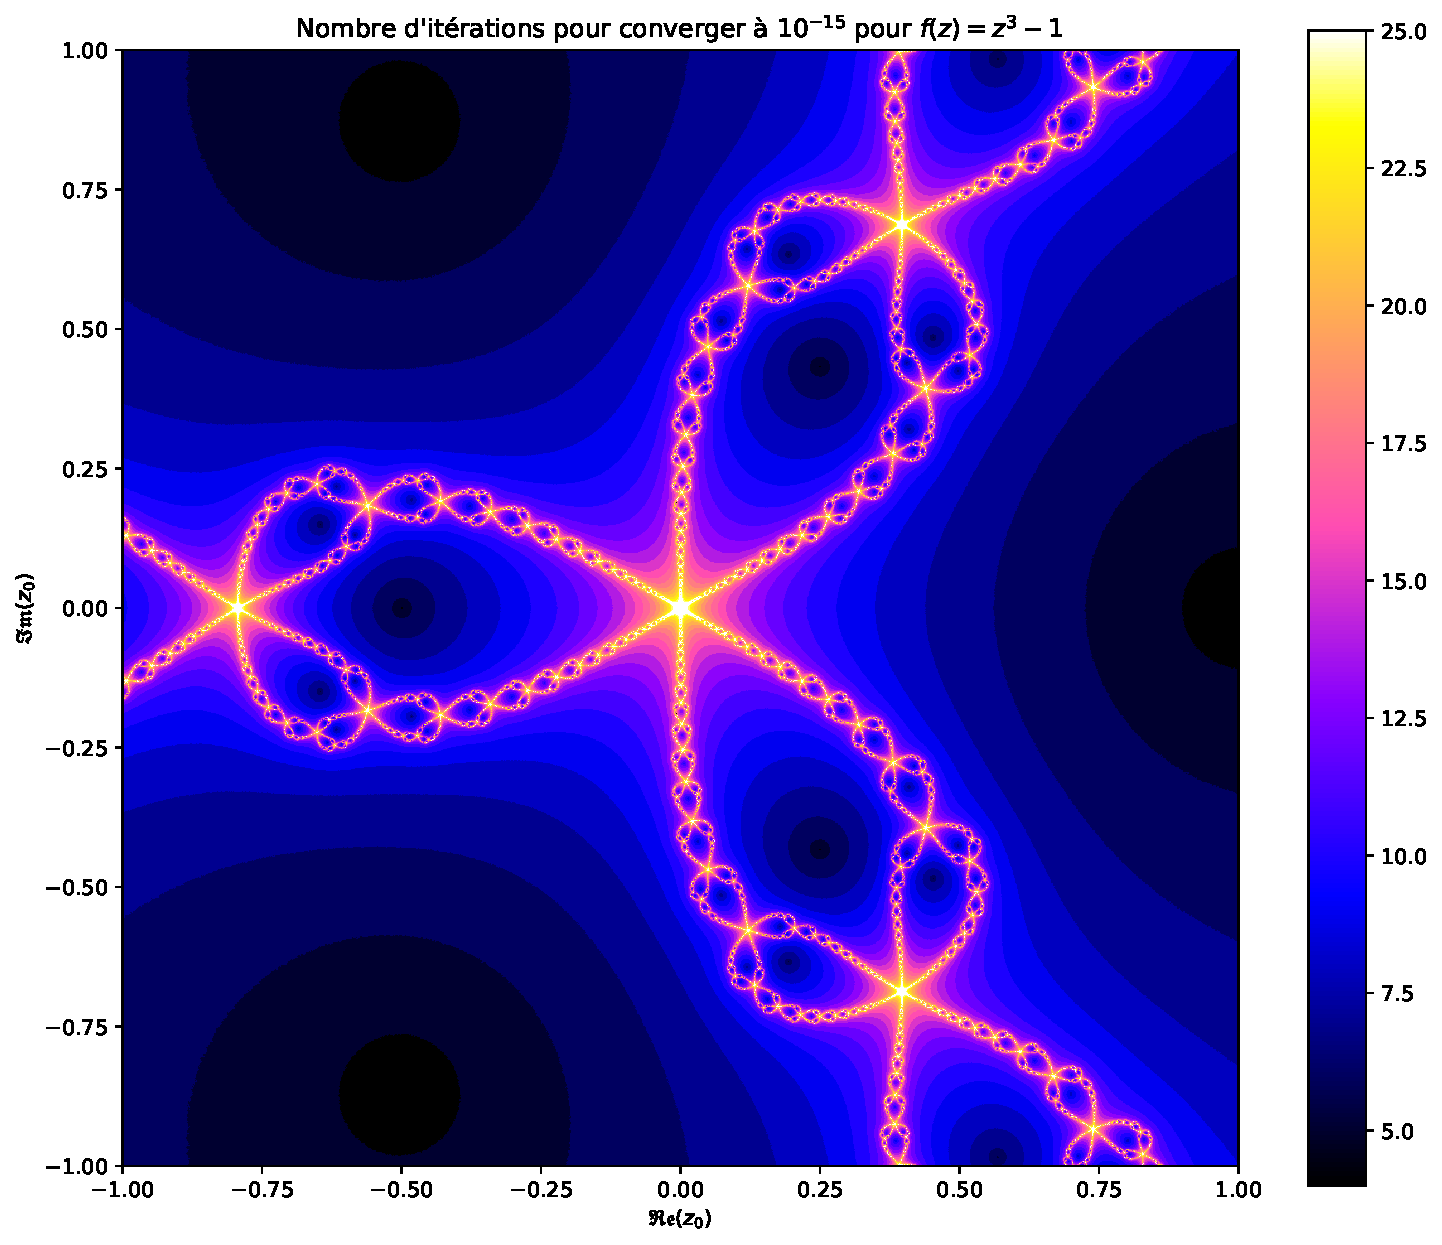
\includegraphics[width=0.95\linewidth]{TD2/newton_newton_niter.a1.pdf}
\end{correction}

\subsection{Amortissement [bonus]}

Avec le polynôme $z^3-1$, on observe une convergence de la méthode de Newton presque partout. Mais il n'est pas garanti que ça soit toujours le cas. Étudions $f(z)=z^4-2z^2-1$. Combien de zéros ce polynôme a-t-il ? Au lieu de déterminer les zéros à la main, on va laisser notre programme le faire... puisque c'est justement l'utilité de la méthode de Newton. Modifiez le programme pour découvrir les zéros au fil du parcours de la grille. Retracez une carte des bassins de convergence pour ce nouveau polynôme. Avons-nous toujours convergence (quelque soit \inline{max_it}) partout ?\\

\begin{correction}
Remplaçons notre tableau statique de zéros par un tableau dynamique :
\begin{minted}[breaklines,samepage]{c++}
  std::vector<complexe> zeros;
\end{minted}
Il suffit d'adapter le code de détermination du numéro du zéro pour ajouter un éventuel nouveau zéro à la liste. Par exemple :
\begin{minted}[breaklines,samepage]{c++}
  // détermination du numéro du zéro
  int num_zero = -1;
  if (nit >= 0) {
    for (int k = 0; k < zeros.size(); k++) {
      if (std::norm(z_zero-zeros[k]) < 1e-10)
        num_zero = k;
    }
    if (num_zero == -1) {
      zeros.push_back(z_zero);
      num_zero = zeros.size() - 1;
    }
  }
\end{minted}
On rajoute bien sûr une quatrième couleur à notre programme Python. On obtient :
\begin{center}
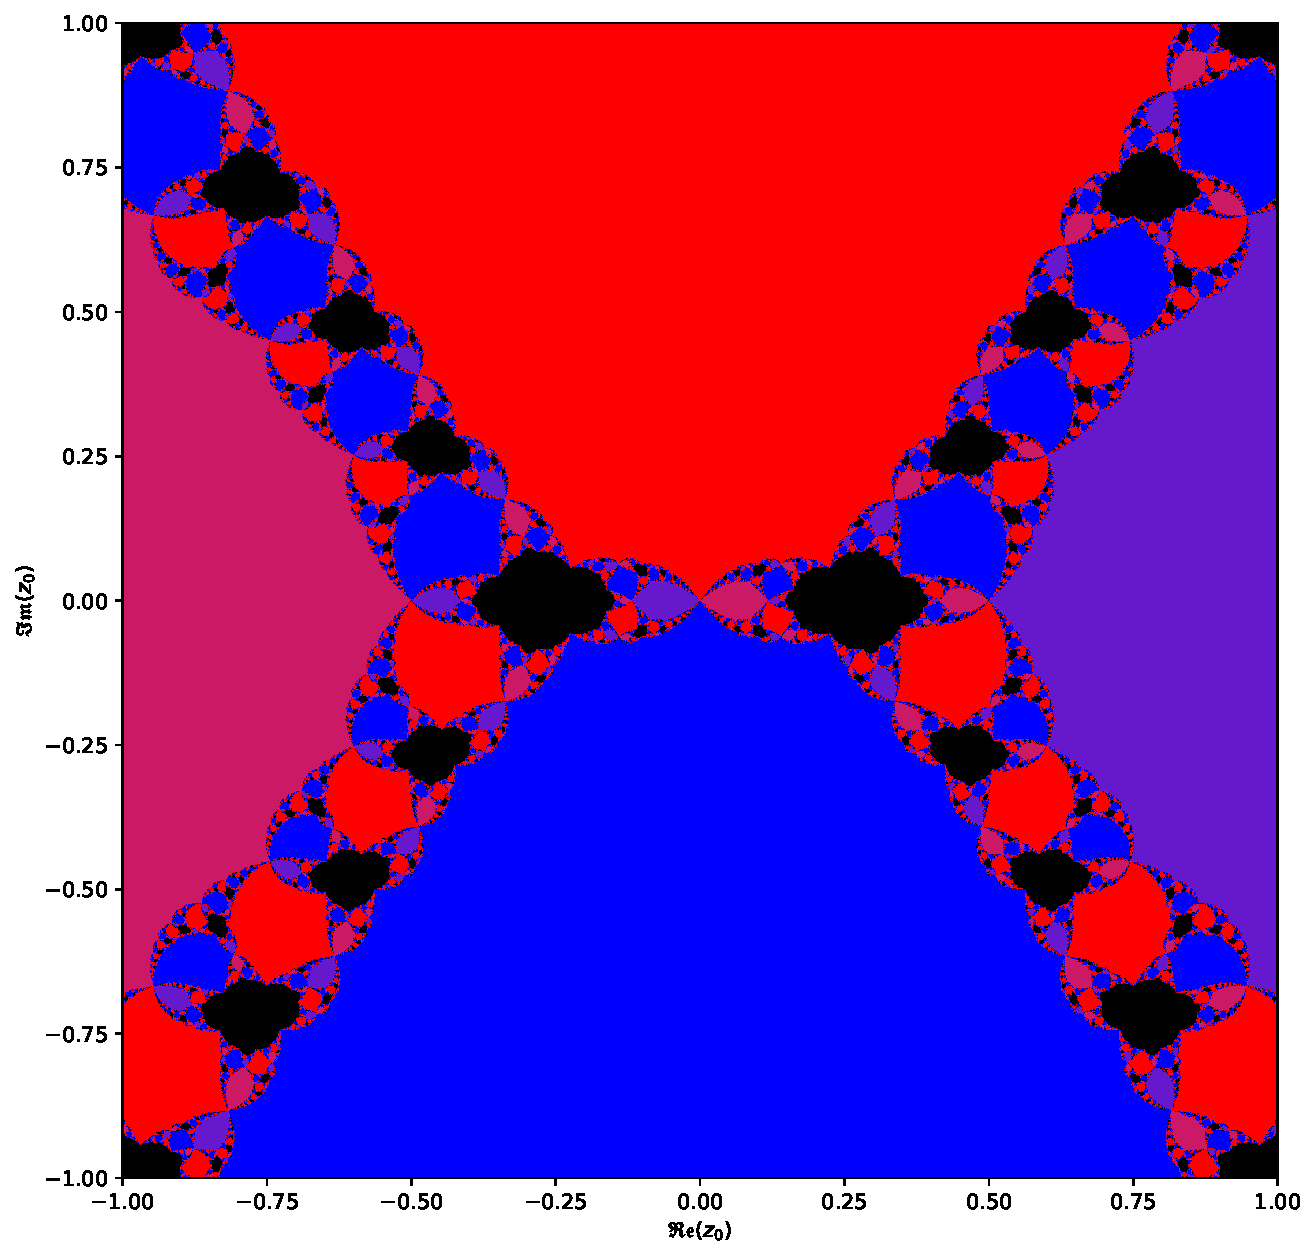
\includegraphics[width=0.7\linewidth]{TD2/newton_bassins_converg_z4_2z2_1.h1.pdf}
\end{center}
On remarque des zones, ici en noir, où la méthode de Newton ne converge jamais. Elle oscille en fait entre deux lobes noirs indéfiniement.
\end{correction}

Remplaçons la relation de récurrence de la méthode de Newton par une version amortie
\begin{equation*}
z_{n+1} = z_n - h\cdot\frac{f(z_n)}{f'(z_n)}
\end{equation*}
où $h\in\,]0,1]$. On parle d'amortissement car à chaque itération, le pas $|z_{n+1}-z_n|$ est plus petit quand $h<1$.\\

Modifiez votre programme et retracez une carte des bassins de convergence. Comme la méthode est nécessairement plus lente à converger, il peut être nécessaire d'augmenter le nombre d'itérations maximales. Qu'observez-vous ? En quoi cela peut-il est considéré comme une amélioration ?

\begin{correction}
Même avec un amortissement modeste de $h=0.8$, on élimine totalement les oscillations de la méthode de Newton (pour cette fonction du moins), et on a une convergence presque partout :
\begin{center}
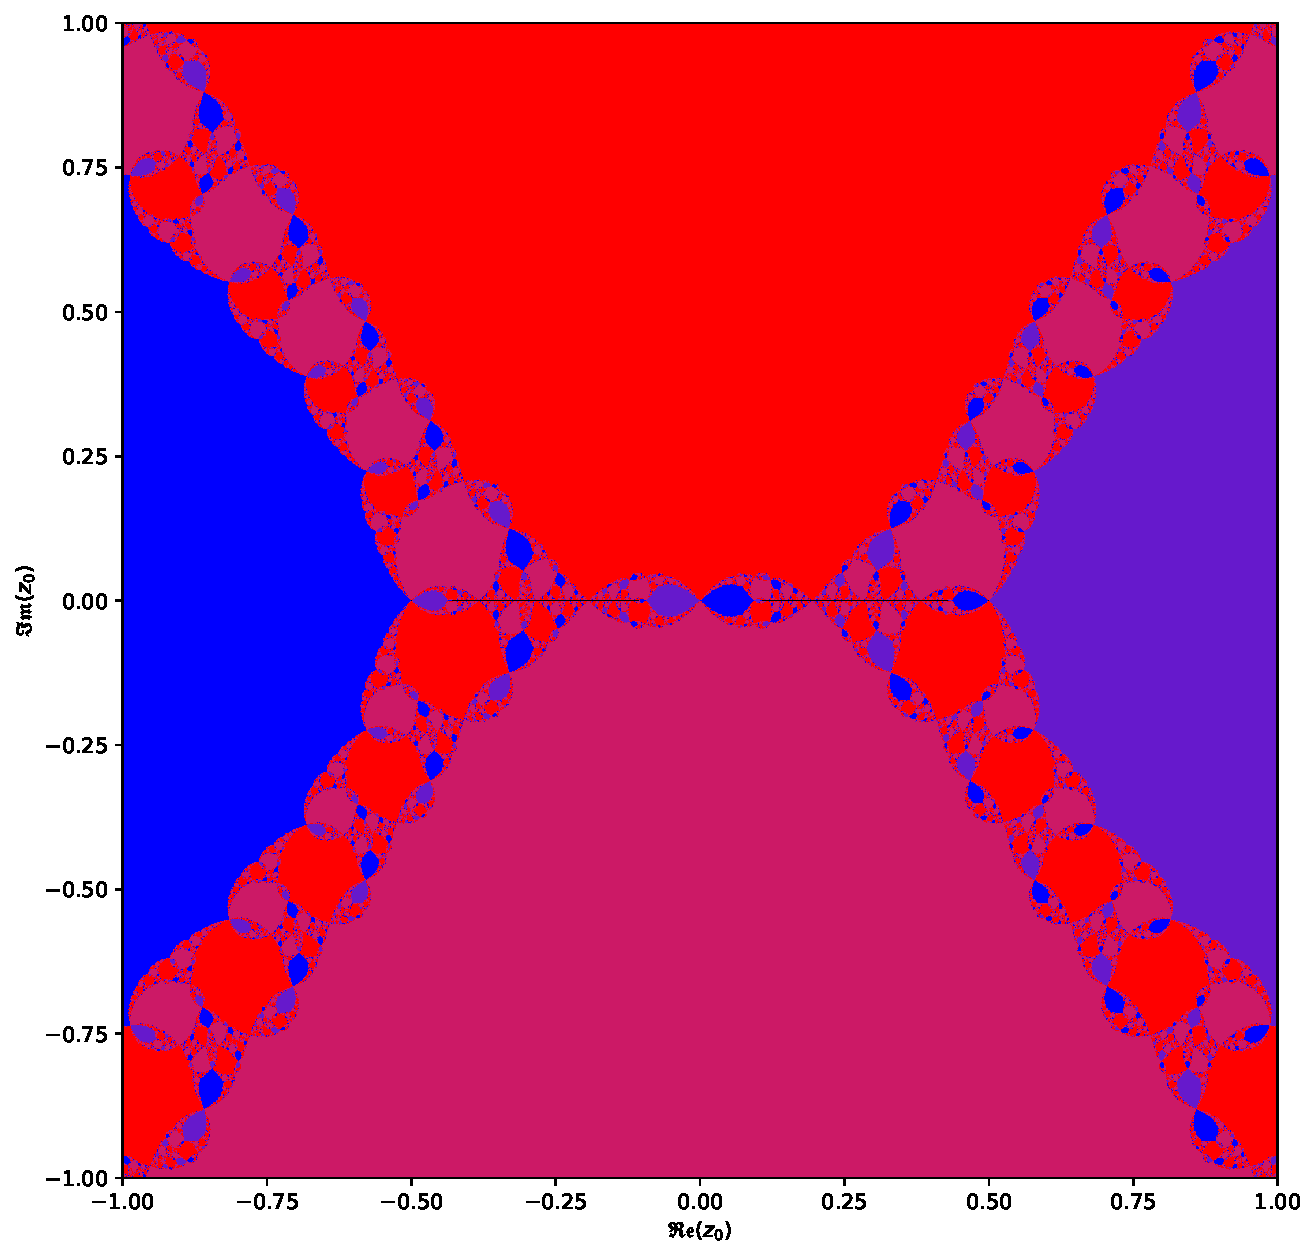
\includegraphics[width=0.7\linewidth]{TD2/newton_bassins_converg_z4_2z2_1.h08.pdf}
\end{center}
Au vu du faible ralentissement induit par cet amortissement, il est clairement avantageux de l'introduire pour améliorer les propriétés de convergence de la méthode de Newton.\\

Pour conclure, revenons à $f(z)=z^3-1$. Voici les bassins de convergence pour $a=1$, et pour des facteurs d'amortissement de $h=0.1$ (gauche; nécessite d'augmenter le nombre d'itérations à 200 pour $\epsilon=10^{-8}$) et $h=0.01$ (droite; nécessite d'augmenter le nombre d'itérations à 2000 pour $\epsilon=10^{-8}$) :
\begin{center}
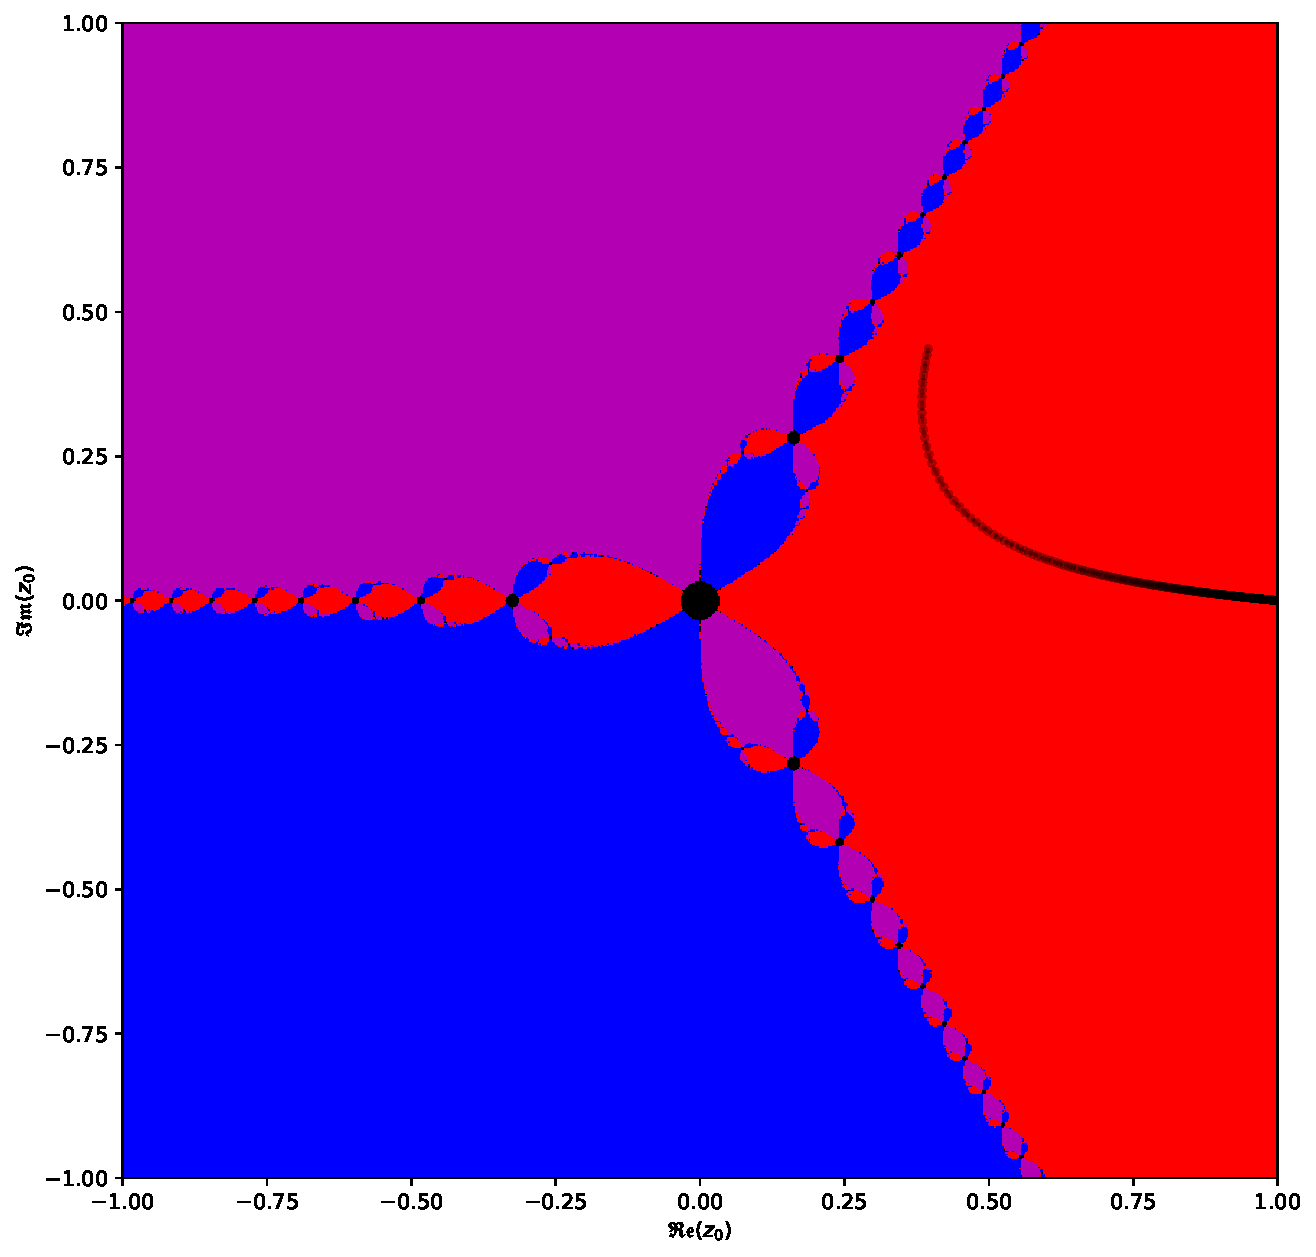
\includegraphics[width=0.49\linewidth]{TD2/newton_bassins_converg.a1.h01.pdf}
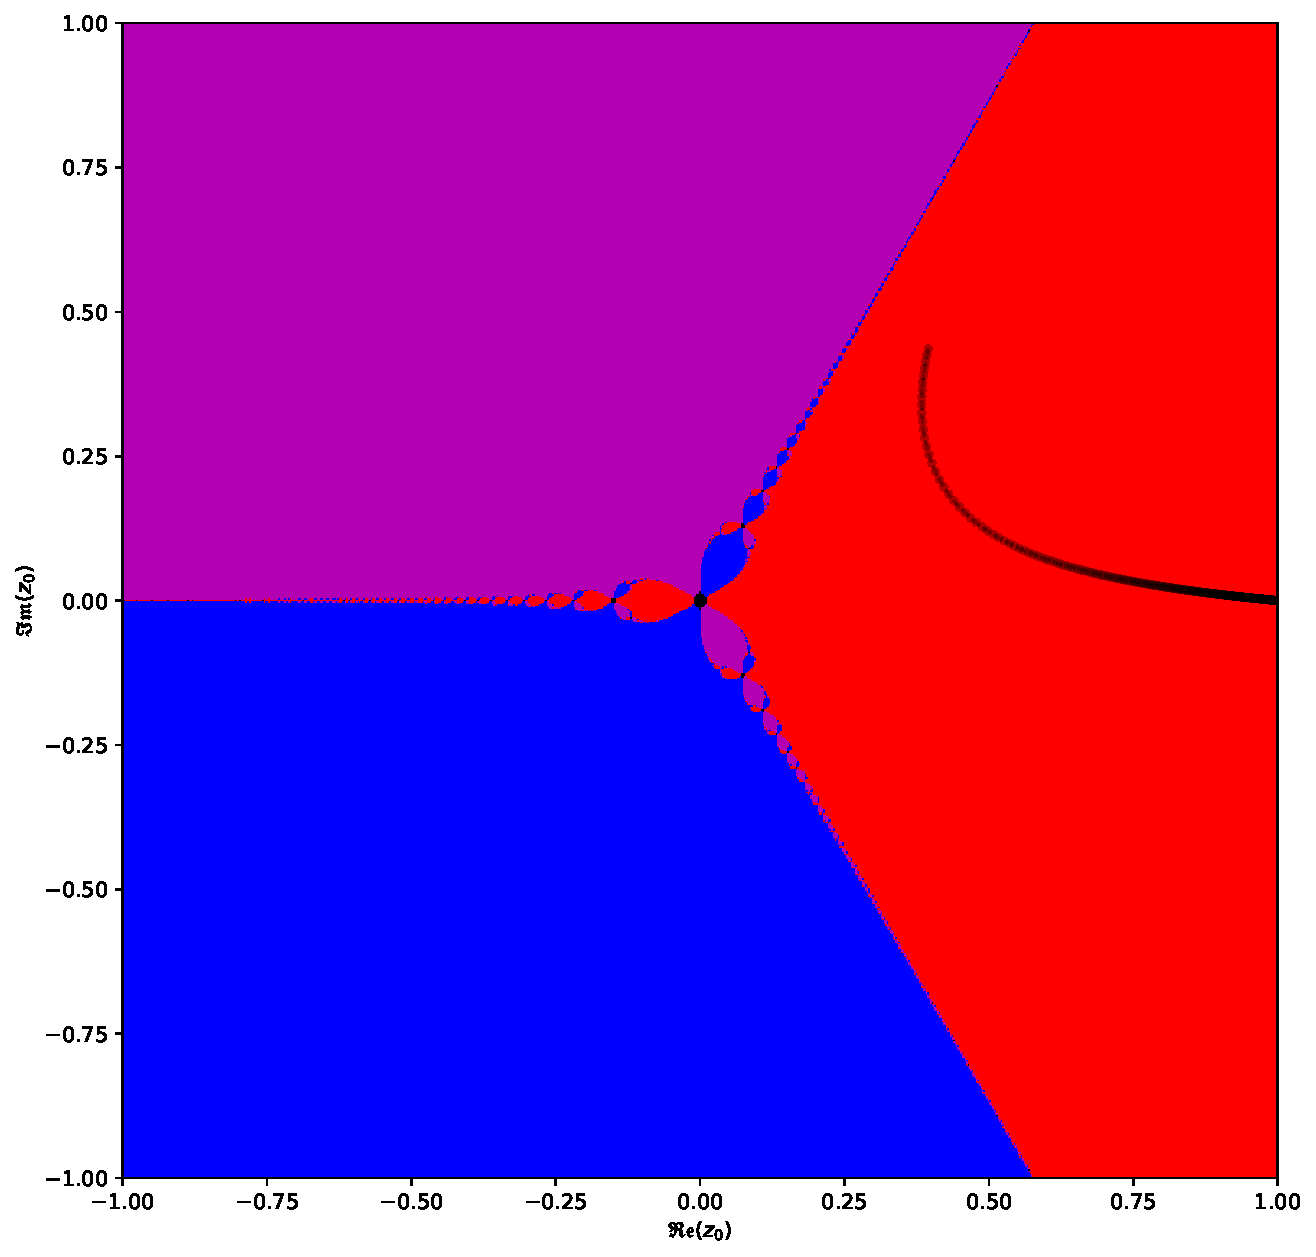
\includegraphics[width=0.49\linewidth]{TD2/newton_bassins_converg.a1.h001.pdf}
\end{center}
On voit que les zones chaotiques diminuent en taille. Cela veut dire que le zéro que l'on va obtenir est bien plus prévisible. On remarque en fait que les bassins de convergence se rapprochent des "bassins versants" (au sens de l'écoulement de l'eau sur une surface $|f(z)|$ vers les zéros). Tracez $|f(z)|$ pour vous en convaincre. Pour $h \ll 1$, on effectue en fait une descente de gradient, qui est beaucoup moins efficace mais aussi beaucoup plus prédictible.
\end{correction}

\end{document}
